%% 
%% Copyright 2007-2024 Elsevier Ltd
%% 
%% This file is part of the 'Elsarticle Bundle'.
%% ---------------------------------------------
%% 
%% It may be distributed under the conditions of the LaTeX Project Public
%% License, either version 1.3 of this license or (at your option) any
%% later version.  The latest version of this license is in
%%    http://www.latex-project.org/lppl.txt
%% and version 1.3 or later is part of all distributions of LaTeX
%% version 1999/12/01 or later.
%% 
%% The list of all files belonging to the 'Elsarticle Bundle' is
%% given in the file `manifest.txt'.
%% 
%% Template article for Elsevier's document class `elsarticle'
%% with harvard style bibliographic references

\documentclass[preprint,12pt]{elsarticle}

%% Use the option review to obtain double line spacing
%% \documentclass[preprint,review,12pt]{elsarticle}

%% Use the options 1p,twocolumn; 3p; 3p,twocolumn; 5p; or 5p,twocolumn
%% for a journal layout:
%% \documentclass[final,1p,times]{elsarticle}
%% \documentclass[final,1p,times,twocolumn]{elsarticle}
%% \documentclass[final,3p,times]{elsarticle}
%% \documentclass[final,3p,times,twocolumn]{elsarticle}
%% \documentclass[final,5p,times]{elsarticle}
%% \documentclass[final,5p,times,twocolumn]{elsarticle}

%% For including figures, graphicx.sty has been loaded in
%% elsarticle.cls. If you prefer to use the old commands
%% please give \usepackage{epsfig}

%% The amssymb package provides various useful mathematical symbols
\usepackage{amssymb}
%% The amsmath package provides various useful equation environments.
\usepackage{amsmath}
%% The amsthm package provides extended theorem environments
%% \usepackage{amsthm}

%% The lineno packages adds line numbers. Start line numbering with
%% \begin{linenumbers}, end it with \end{linenumbers}. Or switch it on
%% for the whole article with \linenumbers.
%% \usepackage{lineno}

%\usepackage[utf8]{inputenc}
%\usepackage[T1]{fontenc}
\usepackage{gensymb}
\usepackage{algorithm}
\usepackage{algorithmic}
\usepackage{multirow}
\usepackage{enumerate}

\journal{Engineering Applications of Artificial Intelligence}

\begin{document}

\begin{frontmatter}

%% Title, authors and addresses

%% use the tnoteref command within \title for footnotes;
%% use the tnotetext command for theassociated footnote;
%% use the fnref command within \author or \affiliation for footnotes;
%% use the fntext command for theassociated footnote;
%% use the corref command within \author for corresponding author footnotes;
%% use the cortext command for theassociated footnote;
%% use the ead command for the email address,
%% and the form \ead[url] for the home page:
%% \title{Title\tnoteref{label1}}
%% \tnotetext[label1]{}
%% \author{Name\corref{cor1} \fnref{label2}}
%% \ead{email address}
%% \ead[url]{home page}
%% \fntext[label2]{}
%% \cortext[cor1]{}
%% \affiliation{organization={},
%%             addressline={},
%%             city={},
%%             postcode={},
%%             state={},
%%             country={}}
%% \fntext[label3]{}

\title{Forecasting the Trajectory of Personal Watercrafts Using Models Based on Recurrent Neural Networks} %% Article title

%% use optional labels to link authors explicitly to addresses:
%% \author[label1,label2]{}
%% \affiliation[label1]{organization={},
%%             addressline={},
%%             city={},
%%             postcode={},
%%             state={},
%%             country={}}
%%
%% \affiliation[label2]{organization={},
%%             addressline={},
%%             city={},
%%             postcode={},
%%             state={},
%%             country={}}
%AUTHOR 1
\author[1,2]{Lucija \v{Z}u\v{z}i\'{c}}
\ead{lucija.zuzic@uniri.hr}

\author[1,2]{Franko Hr\v{z}i\'{c}}
\ead{franko.hrzic@riteh.uniri.hr}

\author[1,2]{Jonatan Lerga\corref{cor1}}%\fnref[label2]
\ead{jonatan.lerga@riteh.uniri.hr}
 
% Address/affiliation
\affiliation[1]{organization={Department of Computer Engineering, Faculty of Engineering, University of Rijeka},
addressline={Vukovarska 58}, 
%         city={Rijeka},
%citysep={Rijeka}, % Uncomment if no comma needed between city and postcode
postcode={51000 Rijeka}, 
country={Croatia}}

\affiliation[2]{organization={Center for Artificial Intelligence and Cybersecurity, University of Rijeka},
addressline={Radmile Matejcic 2}, 
postcode={51000 Rijeka}, 
country={Croatia}}

%\fntext[label2]{http://www.riteh.uniri.hr/osoba/jonatan-lerga}
% Corresponding author text
\cortext[cor1]{Corresponding author} 

%% Abstract
\begin{abstract}
Monitoring rental boats and predicting the reckless driving behavior of inexperienced motorboat operators in popular tourist destinations is a relatively unexplored field of research since previous work focuses on other types of vehicles and is only applicable to specific maritime traffic routes. By analyzing trajectories from real-world data collected worldwide, we tested and developed multiple versions of a joint location-agnostic model based on deep learning approaches for trajectory forecasting. Firstly, well-known lightweight neural networks, namely RNN (Recurrent Neural Network), LSTM (Long Short-Term Memory), or GRU (Gated Recurrent Unit) models, were tested. Attention mechanism-based models along with the most recently developed foundation model \textbf{Uni}fied \textbf{T}ime \textbf{S}eries (UniTS) for time-series data were added, exploring their potential in this unexplored field. LSTM bidirectional and convolutional models for evaluating peptide sequence self-assembly were also adapted and benchmarked. Longitude, latitude, speed, and heading variables defining trajectories were forecast to make the test robust and directly applicable to the developing monitoring system. Our research showed that the approach based on the foundation model obtained the best results, successfully expanding the utilization of foundation models to the domain of maritime trajectory estimation and eliminating challenging hyperparameter selection required by the other models.
\end{abstract}

%%Graphical abstract
%\begin{graphicalabstract}
%\includegraphics{grabs}
%\end{graphicalabstract}

%%Research highlights
%\begin{highlights}
%\item Comparing an attention mechanism and the UniTS model with RNN, GRU, and LSTM NNs
%\item Developing a joint location-agnostic model on real-world data from multiple sites
%\item Achieving an $R^{2}$ over $90\%$ for trajectories forecasted with the UnitS model
%\item Testing model stability using stratified nested $k$-fold cross-validation
%\end{highlights}

%% Keywords
\begin{keyword}
personal watercraft \sep trajectory forecasting \sep recurrent neural network \sep attention mechanism \sep foundation model
\end{keyword}

\end{frontmatter}

%% Add \usepackage{lineno} before \begin{document} and uncomment 
%% following line to enable line numbers
%% \linenumbers

%% main text
%%

% MAIN TEXT 
\section{Introduction}
%\label{sec:Introduction}
%\vspace{10pt}

At frequently visited tourist destinations, large marines with many ships monitor the rented vehicles, using a personal watercraft tracking system such as the one provided by the company OtoTrak \cite{ototrakOtoTrakTrack}, as inexperienced drivers pose a danger to all participants in marine traffic. In the described system \cite{ototrakOtoTrakTrack}, speed limits are enforced when a driver leaves the specified longitude and latitude zone or approaches another vessel using the same cloud-based personal watercraft tracking system that enables remote vehicle control. The module \cite{ototrakOtoTrakTrack} continuously transmits Global Positioning System (GPS) signals to activate these functions.

Human drivers can correctly assess the future movement of surrounding traffic participants, which is especially important in crowded or narrow areas. Currently developed systems for Advanced Driver Assistance Systems (ADAS), such as Adaptive Cruise Control (ACC) for land vehicles, lack this capability. Such systems are reactive, meaning the driver is still responsible for all decisions while the system provides advanced precautionary measures. Vehicles that are fully autonomous but lacking forecasting capabilities usually have to act cautiously in the presence of other traffic participants to avoid dangerous situations, such as a low-speed collision between a passenger bus and a self-driving car \citep{dolgov2016google}. This proves that accurately forecasting the movements of other vehicles is crucial for autonomous driving.

One possible solution is to learn the vehicle driving patterns and forecast their future movement. Those patterns are hard to learn, evident in highway driving, where long periods of constant speed are interrupted by sudden changes, such as lane changes. In some work, data is handpicked \citep{ding2013neural, zheng2014predicting} or datasets are collected for a specific purpose \citep{kumar2013learning}. This could be an inaccurate representation of real-life situations and negatively affect the performance of the trained model. Real-world data from different locations should be merged to train and test models that can be directly applied to a new region without additional training, as done in this study.

This work aims to forecast the driver's future behavior based on historical data, evaluating deep-learning methods such as various Recurrent Neural Network (RNN) models, including those using a simple RNN or Long Short-Term Memory (LSTM) \citep{hochreiter1997long} and Gated Recurrent Unit (GRU) layers for multiple variables. The use of RNNs for forecasting trajectories for other vehicle types is demonstrated in several papers, including work by Altché and de La Fortelle \citep{altche2017lstm}, which uses LSTM for forecasting vehicle trajectories on highways. LSTMs are particularly well suited for forecasting time series \citep{gers2000learning} as they can memorize previous inputs. Recently, LSTMs have been widely used to forecast vehicle destinations at an intersection \citep{phillips2017generalizable, zyner2017long} and also for pedestrians \citep{duan2016travel, alahi2016social}. We also applied the \textbf{Uni}fied \textbf{T}ime \textbf{S}eries (UniTS) foundation model which has recently been developed and includes an attention mechanism for various time-series tasks and datasets. Inspired by the origin of the UniTS model in Large Language Models (LLMs), we also compared an attention mechanism originally designed for machine translation. Finally, a novel architecture using LSTM bidirectional and convolutional layers, and encoding Aggregation Propensity (AP) of amino acids, dipeptides, and tripeptides and Sequential Properties (SP) of amino acids to predict peptide sequence self-assembly was also used due to similarities in merging multiple arrays of sequential data in different ranges.

The module processes different variables, including latitude and longitude offset, speed, and heading. These variables are measured and forecasted. The latitude and longitude offset is used in one of the trajectory estimation methods proposed in our paper. The second proposed method uses the speed, heading, and the actual time interval between records in the database. The time interval represents the elapsed time between records in the database that form a trajectory for a single trip. As data without transmission errors was scarce, stratified nested $k$-fold cross-validation was used to perform a detailed test of the models. The training, validation, and testing split was stratified to preserve the ratio of trajectories from each vehicle.

The generated forecasts could be used to avoid unnecessary speed limits in non-hazardous situations. It also ensures the safety of drivers and other participants in maritime traffic.

As far as we know, this is the first time deep-learning methods have been applied to personal watercraft trajectory forecasting. The main contributions of this paper are:

\begin{itemize}
    \item Comparing an attention mechanism and the UniTS model with RNN, GRU, and LSTM NNs
    \item Developing a joint location-agnostic model on real-world data from multiple sites
    \item Achieving an $R^{2}$ over $90\%$ for trajectories forecasted with the UnitS model
    \item Testing model stability using stratified nested $k$-fold cross-validation
\end{itemize}

The findings indicate the forecast could be used in real-life systems and support our hypothesis.

The rest of the paper is structured as follows. Other work using machine learning and other algorithms for prediction or anomaly detection in maritime traffic is given in Section~\ref{sec:Related}. The dataset is described in Section~\ref{sec:Dataset}. Section~\ref{sec:Methods} outlines the methodology used in this work. The evaluation metrics are listed in Section~\ref{sec:EvaluationMetrics}. Section~\ref{sec:Results} presents the results obtained in this work. Section~\ref{sec:Discussion} discusses the implications of the results. The main points are summarised and the conclusion is given in Section~\ref{sec:Conclusion}.

\section{Related Work}
\label{sec:Related}
%\vspace{10pt}

An overview of motion forecasting in the scientific literature \citep{lefevre2014survey} shows that, as with other machine learning applications, the methodology can be divided into classification or regression methods.

Classification problems in motion forecasting are concerned with forecasting a higher-level intention, such as the direction of a turn at an intersection. Hidden Markov models \citep{tay2012probabilistic, streubel2014prediction}, Kalman filtering \citep{carvalho2014stochastic}, support vector machines \citep{mandalia2005using, kumar2013learning} or a vehicle model \citep{houenou2013vehicle} have been used for this purpose. Artificial neural networks \citep{yoon2016multilayer, khosroshahi2016surround, phillips2017generalizable} have recently been increasingly used. Discrete outputs facilitate the training and evaluation of models for behavior forecasting. On the other hand, the information provided is scarce and difficult to use to create a trajectory. Gaussian processes \citep{tay2012probabilistic} or neural networks \citep{yoon2016multilayer} have been used in generative models based on the output of behavior forecasting. This requires training multiple models and is dependent on the accuracy and robustness of the classifier. We did not have access to labeled data in this paper, so applying classification models would be challenging as any generated labels would not have empirical evidence to support them.

Olensen et. al. \cite{olesen2023contextually} apply two-step clustering based on positions and kinematics of vessels to detect anomalies in a region of interest without previous labels in an unsupervised manner less computationally intensive and more interpretable than neural networks. However, this model is location-dependent, and kinematic anomalies might be difficult to detect in faster smaller vessels. The proposed model uses forecasting rather than labeling and does not rely on a single region of interest to expand applicability.

Solutions to regression problems provide a direct estimation of future positions that can be used to generate trajectories. Regression algorithms such as regression forests \citep{volz2016predicting} are applicable. Artificial neural networks have attracted the most attention and have been used for forecasting the movement of pedestrians \citep{duan2016travel, alahi2016social}, cars \citep{tomar2012safety, liu2014vehicle} or cyclists \citep{zernetsch2016trajectory}. Dynamic neural network models, such as the nonlinear autoregressive exogenous model (NARX), perform better than static feed-forward neural networks when used to create a forecasting model for a constantly changing system, such as the speed output of the GEROLER motor \citep{gregov2022modeling}, demonstrating the importance of model novelty. The lack of a confidence measure is a major shortcoming of these approaches. Monte Carlo sampling or $k$-fold validation \citep{fushiki2011estimation} is used for error estimation and can mitigate this problem. Dropout can be applied in neural networks \citep{gal2016dropout} with the same motivation, but this was not done in the tested models. Model stability was instead extensively examined using stratified nested $k$-fold cross-validation.

A study by Venskus et al. \cite{venskus2021unsupervised} uses an LSTM network for unsupervised prediction region learning to detect anomalies as movement outside this region. However, such a model would need to be retrained for new locations, while the model proposed in this study can be applied as-is, providing an out-of-the-box solution to predict the future movement of vessels. Additionally, the proposed model does not predict only the region's upper and lower bounds but fully describes independent and unrestricted movement.

Graph neural networks are a separate category of models that have recently been widely applied to maritime traffic \cite{jiang2022graph, jiang2023graph}. However, these models are intended for maritime routes and other systems that can be modeled as graphs. Personal watercraft used in this study do not rely on predefined traffic patterns. The trajectories of these vessels do not have a fixed origin point and destination. Movement is not regulated except for the reachable range without refueling, natural boundaries, or paid-for rental time. As such, graph neural networks are not suited to this problem, but should be used for cargo, industrial, and mass passenger vessels.

\section{Dataset}
\label{sec:Dataset}
%\vspace{10pt}

The utilized database \cite{ototrakOtoTrakTrack} contains information about the rental locations, the vehicles, and the data recorded for each trip, including speed, heading, latitude, and longitude. The trajectories of the vessels were recorded in Croatia, Spain, Portugal, Greece, Canada, and the United States of America in July 2023 when most of the mentioned countries hit the peak of tourist season, and therefore the increased personal watercraft presence. All of this data for each tested variable was jointly fed into a single unified version of a model for training, testing, and validation. In addition, all trajectories flagged by the system as containing errors or large gaps in transmission were excluded. The "ERROR" flag means that recordings are missing, while in "TRACKING" mode recordings in the database are sent less frequently. These large gaps in communication could be filled by interpolation in a real-life system. The models were trained and tested on original data to preserve integrity.  The usual frequency of report transmission is one second, which means that only one second has elapsed between two points in time recorded by the monitoring system.

The utilized system identifies data from the same trajectory using unique ride and vehicle numbers. A unique vehicle number identifies a personal watercraft that can be used multiple times in different trajectories or trips. The vehicle number is important because the same vehicle is always rented and used at the same location. A unique trip number identifies a trajectory constructed in a trip with a rented personal watercraft, identified by its unique vehicle number.

\subsection{Preprocessing}
%\label{subsec:Preprocessing} 
%\vspace{10pt}

Four variables were separately forecast by the models created in this work. These variables are speed, heading, longitude, and latitude offset. In this work, the trajectories are defined by different subsets of the investigated variables, necessary to describe the movement in two-dimensional space. These subsets were either longitude and latitude offset or speed and heading. The elapsed time between two records in the database or the distance between two points in time was not forecast but used to create a full trajectory from speed and heading.

To boost performance and mitigate problems that may arise due to the varying magnitudes among different parts of the input data~\cite{singh2020investigating, nawi2013effect}, several conventions were proposed to unify and normalize the data:

\begin{enumerate}[i]
  \item The values for latitude and longitude are rounded to ten decimal places to obtain a finite state space.
  \item The speed at the point is recorded in kilometers per hour and rounded to a whole number.
  \item The heading, i.e. the offset from the North ($90\degree$, positive direction of the $y$ axis), which has a value between $0\degree$ and $360\degree$, recorded by the module and increases from east to west, was also used.
  \item The time between two recorded points was also modeled and rounded to milliseconds, i.e. seconds with three decimal places.
  \item For each trajectory, the latitudes and longitudes were converted into relative values, i.e. distances from the starting point to ensure the model is location-independent. The latitudes and longitudes were further normalized to a range of $0.1$ $\degree$ of latitude and longitude, as no trajectory was found in the data used that covered a larger range than this.
  \item Trajectories on the negative side of the $x$ axis are mirrored on the $y$ axis, and trajectories on the negative side of the $y$ axis are mirrored on the $x$ axis. An example of the calculation of the $x$ and $y$ offset at three consecutive points of a trajectory can be seen in Figure~\ref{fig:actual}.
\end{enumerate}

\begin{figure}[!ht]
    \centering
    \includegraphics[width =0.99 \linewidth]{actual.png}
    \caption{Calculating $x$ and $y$ offset.}
    \label{fig:actual}
\end{figure}

After preprocessing, the distributions of $x$ and $y$ offset are centered around zero, and the time between records is centered around $1$ $s$, as visible in the statistical properties in Table~\ref{tab:q1q2q3var} and Table~\ref{tab:miniavgmaxivar}, and the histograms in Figure~\ref{fig:all_var_hist}. In contrast, heading is approximately uniformly distributed across a $360\degree$ range. A linear or exponential function could describe the frequency of speeds which is considerably smaller for higher than for lower speeds.

\begin{table}[!ht]
    \centering
    \begin{tabular}{|c|c|c|c|} 
        \hline
        Variable & $1^{st}$ quartile & Median & $3^{rd}$ quartile \\ \hline
        Heading & $90$ & $188$ & $275$ \\ \hline
        $y$ offset & $-2.16 \times 10^{-4}$ & $1.6 \times 10^{-5}$ & $2.33 \times 10^{-4}$ \\ \hline
        $x$ offset & $-2.5 \times 10^{-4}$ & $5 \times 10^{-5}$ & $3.18 \times 10^{-4}$ \\ \hline
        Speed & $8$ & $17$ & $34$ \\ \hline
        Time ($s$) & $0.94$ & $0.995$ & $1.058$ \\ \hline
    \end{tabular}
    \caption{The $1^{st}$ quartile, median, and $3^{rd}$ quartile for for speed, heading, $x$ and $y$ offset, and time between records after preprocessing.}
    \label{tab:q1q2q3var}
\end{table}

\begin{table}[!ht]
    \centering
    \begin{tabular}{|c|c|c|c|} 
        \hline
        Variable & Minimum & Mean & Maximum \\ \hline
        Heading & $0$ & $180.88672$ & $360$ \\ \hline
        $y$ offset & $-4.783 \times 10^{-3}$ & $2.0841 \times 10^{-5}$ & $2.1183 \times 10^{-2}$ \\ \hline
        $x$ offset & $-1.1634 \times 10^{-2}$ & $2.9387 \times 10^{-5}$ & $9.45 \times 10^{-3}$ \\ \hline
        Speed & $0$ & $22.5432$ & $83$ \\ \hline
        Time ($s$) & $0.001$ & $1.0028$ & $4.735$ \\ \hline
    \end{tabular}
    \caption{The minimum, mean, and maximum measured for speed, heading, $x$ and $y$ offset, and time between records after preprocessing.}
    \label{tab:miniavgmaxivar}
\end{table}

\begin{figure}[!ht]
    \centering
    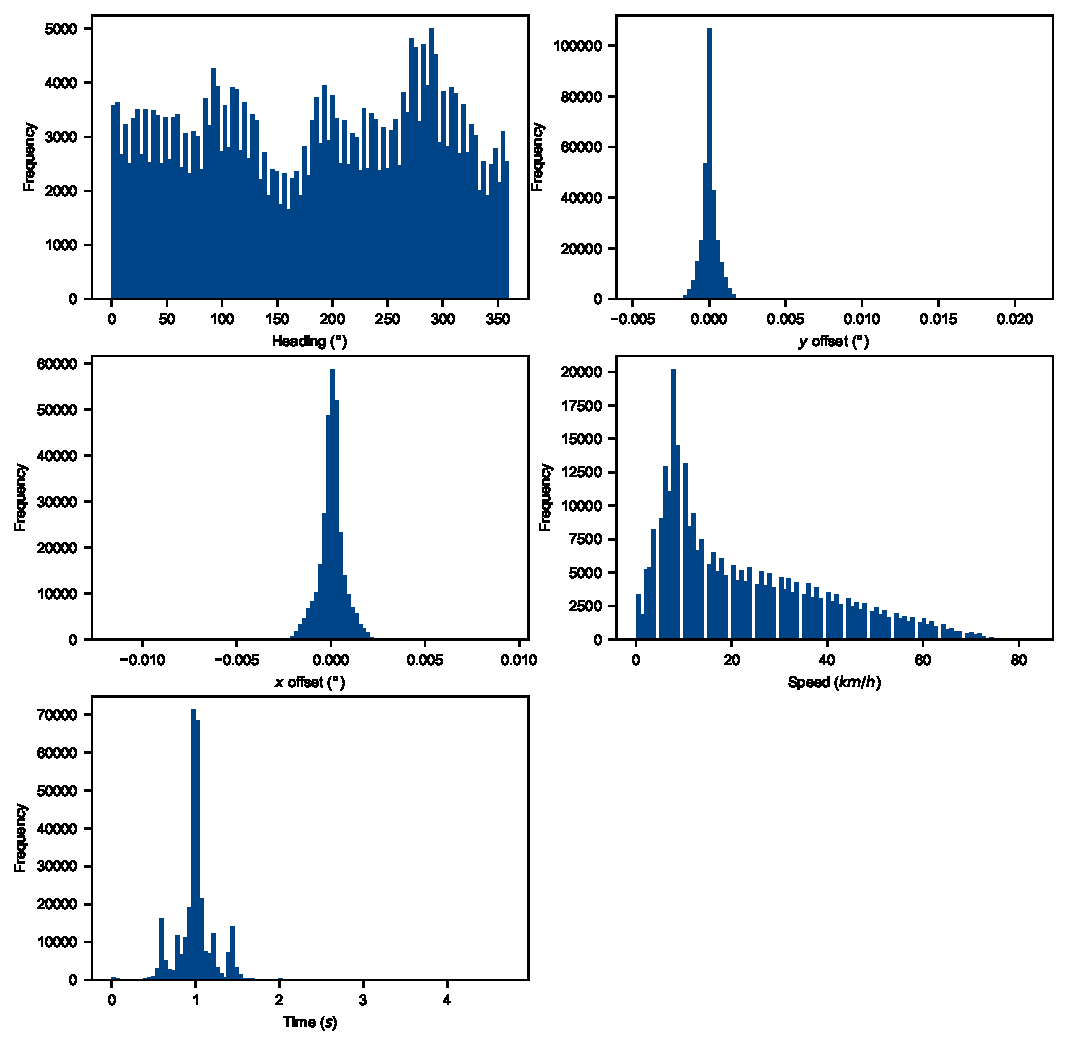
\includegraphics[width =0.99 \linewidth]{all_var_hist.pdf}
    \caption{Histograms of speed, heading, $x$ and $y$ offset, and time between records after preprocessing.}
    \label{fig:all_var_hist}
\end{figure}

\subsection{Estimating a Trajectory}
%\label{subsec:EstimatingTrajectory}
%\vspace{10pt}

The latitude and longitude must be calculated to estimate the trajectory based on the given values of the individual variables. The offsets in the $x$ and $y$ directions can be directly combined to create a trajectory.

An alternative is using speed and heading to obtain offset indirectly. An example of using this method to estimate a trajectory based on the speed, heading, and actual time interval between each pair of records at three consecutive points of a trajectory is shown in Figure~\ref{fig:long speed dir}. Before calculating the values of trigonometric functions, the heading must be subtracted from the offset of $90\degree$ which represents the North, and further transformed according to previously described trajectory mirroring. The elapsed time is used together with the speed to calculate the distance traveled.

\begin{figure}[!ht]
    \centering
    \includegraphics[width = 0.9 \linewidth]{long speed dir.png}
    \caption{Trajectory estimation using speed, heading, and the actual time interval.}
    \label{fig:long speed dir}
\end{figure}
 
A conversion of the units is necessary because the speeds are given in $km/h$ and the longitudes and latitudes in $\degree$. For the latitudes of the processed locations, $1\degree$ latitude and longitude correspond to approximately $111$ $km$, and longitude and latitude were scaled to a range of $0.1$ $\degree$ in this work. The speeds of the module are divided by $111 \times 0.1 \times 3600 = 39960$ to obtain values in $\degree / s$ when estimating a trajectory using values predicted by models.

\subsection{Training, Validation, and Test Datasets}
%\label{subsec:TrainTestValidate} 
%\vspace{10pt}

The used trajectories contained a minimum of $40$, a maximum of $3647$, and an arithmetic mean of $798.583$ points, as visible in the histogram in Figure~\ref{fig:all_traj_features_time}, and in the statistical properties in Table~\ref{tab:q1q2q3var} and Table~\ref{tab:miniavgmaxivar}. A quarter of the trajectories had less than $315$ points, and half were shorter than $693$. Only a quarter of the trajectories were longer than $1189$, and the total number of points in all trajectories was $306656$.

The trajectories covered a range of $36.0605$ $\degree$ longitude, $24.9798$ $\degree$ latitude, and an area of $3.7269$ $\degree$$^{2}$ in total after preprocessing which translated all trajectories to a starting $0$ $x$ and $y$ coordinate, scaled them to a range of $0.1$ $\degree$, and mirrored them to eliminate negative values. The final longitude and latitude ranges are converted to values between $0$ and $1$, where $1$ equals $0.1$ $\degree$.

The distributions of the longitude and latitude ranges and the total area are centered around zero, as visible in the statistical properties in Table~\ref{tab:q1q2q3traj} and Table~\ref{tab:miniavgmaxitraj}, and the histograms in Figure~\ref{fig:all_traj_features_time}. The arithmetic mean is larger than the median, so the number of points and duration are skewed towards lower values. The duration is almost the same as the number of points since $1$ $s$ is the expected time between records in the database.

\begin{table}[!ht]
    \centering
    \begin{tabular}{|c|c|c|c|} 
        \hline
        Variable & $1^{st}$ quartile & Median & $3^{rd}$ quartile \\ \hline
        Number of points & $315$ & $693$ & $1189$ \\ \hline
        Duration ($s$) & $313.9438$ & $694.433$ & $1187.6845$ \\ \hline
        Longitude range ($\degree$) & $3.8767 \times 10^{-2}$ & $7.3683 \times 10^{-2}$ & $1.0932 \times 10^{-1}$ \\ \hline
        Latitude range ($\degree$) & $2.1996 \times 10^{-2}$ & $5.5234 \times 10^{-2}$ & $8.6517 \times 10^{-2}$ \\ \hline
        Total area ($\degree$$^{2}$) & $8.1744 \times 10^{-4}$ & $4.511 \times 10^{-3}$ & $8.2884 \times 10^{-3}$ \\ \hline
    \end{tabular}
    \caption{The $1^{st}$ quartile, median, and $3^{rd}$ quartile for the number of points, duration, longitude and latitude range, and total area covered by trajectories after preprocessing.}
    \label{tab:q1q2q3traj}
\end{table}

\begin{table}[!ht]
    \centering
    \begin{tabular}{|c|c|c|c|} 
        \hline
        Variable & Minimum & Mean & Maximum \\ \hline
        Number of points & $40$ & $798.583$ & $3647$ \\ \hline
        Duration ($s$) & $38.323$ & $799.8493$ & $3646.783$ \\ \hline
        Longitude range ($\degree$) & $3.634 \times 10^{-3}$ & $9.3907 \times 10^{-2}$ & $7.3868 \times 10^{-1}$ \\ \hline
        Latitude range ($\degree$) & $1.267 \times 10^{-3}$ & $6.5051 \times 10^{-2}$ & $9.2658 \times 10^{-1}$ \\ \hline
        Total area ($\degree$$^{2}$) & $1.1509 \times 10^{-5}$ & $9.7055 \times 10^{-3}$ & $1.8796 \times 10^{-1}$ \\ \hline
    \end{tabular}
    \caption{The minimum, mean, and maximum measured for the number of points, duration, longitude and latitude range, and total area covered by trajectories after preprocessing.}
    \label{tab:miniavgmaxitraj}
\end{table}

\begin{figure}[!ht]
    \centering
    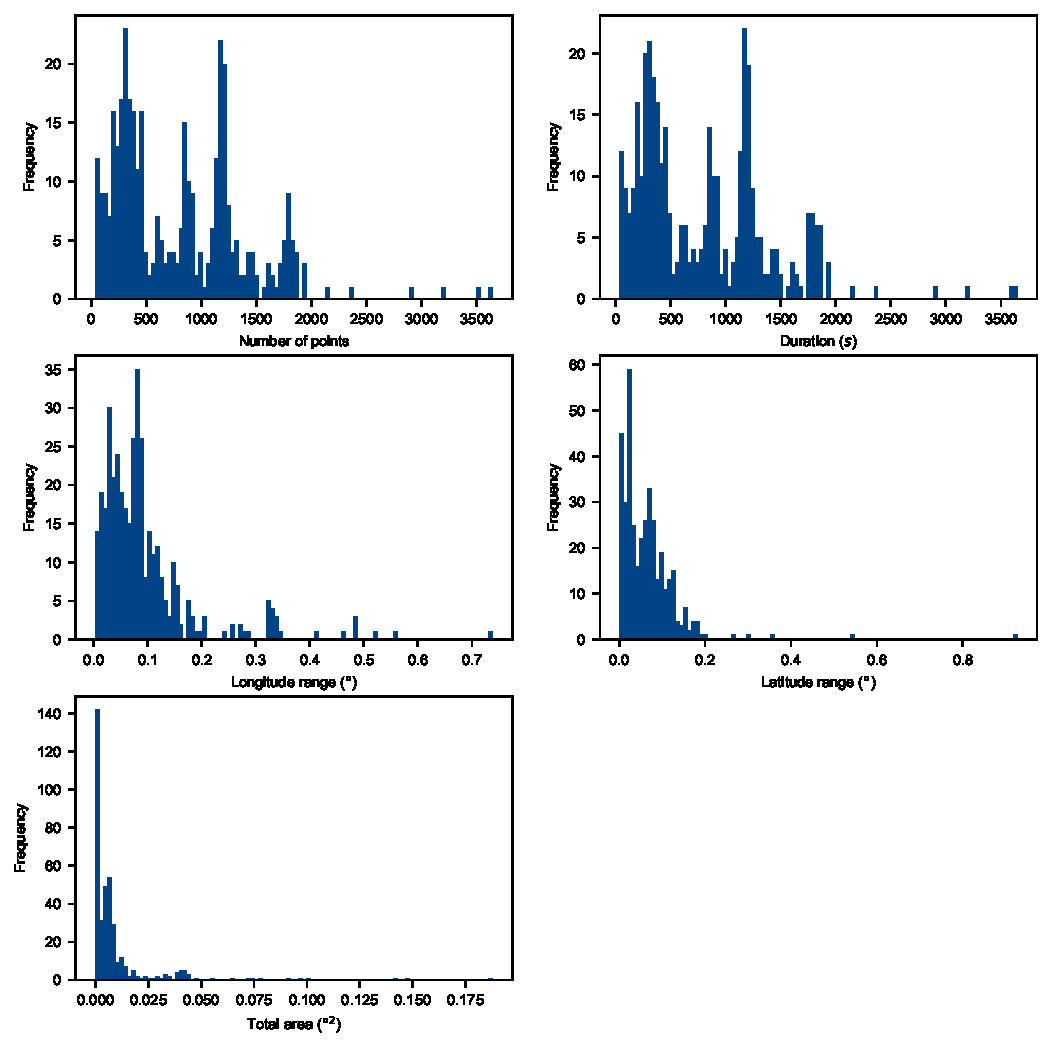
\includegraphics[width =0.99 \linewidth]{all_traj_features_time.pdf}
    \caption{Histograms of the number of points, duration, longitude and latitude ranges, and total area of trajectories after preprocessing.}
    \label{fig:all_traj_features_time}
\end{figure}

The US101 dataset, used by Altché and de La Fortelle \citep{altche2017lstm} for an architecture similar to the one utilized in this study, contains $45$ $min$ in each trajectory for more than $6000$ individual land vehicles for a total of $270000$ $min$. This is significantly more than what is contained in the dataset used in this experiment. Due to the small number of watercraft trajectories available, covering only $307142.119$ $s$ in total, the generated models in this study were extensively tested to confirm stability. Nested $k$-fold cross-validation \cite{fushiki2011estimation} with $5$ testing folds and $5$ validation folds separated from the training data for each testing fold was used to generate $25$ training, testing, and validation splits. A fixed random seed was used when generating the splits to ensure reproducibility across multiple function calls. The splits were stratified to ensure that the same ratio of trajectories from each vehicle was present in the training, validation, and testing data. Each training fold contained $246$ or $247$ trajectories, each testing fold contained $76$ or $77$ trajectories, and each validation fold contained $61$ or $62$ trajectories. The sizes of folds are not equal since the total number of trajectories is not divisible by $5$, the number of folds used, but the difference in the size of any two folds is never larger than one.

\section{Methods}
\label{sec:Methods}
%\vspace{10pt}

This section briefly describes the structure of the models used to forecast vessel position. We used RNN models with simple RNN, LSTM, or GRU layers in four different architectures, later referred to as the "Reference", "Linear", "Twice", and "Third" models, for a total of $12$ models. A GRU attention model with four hyperparameter experiment settings and the UniTS foundation model is also used. This brings the total number of tested models up to $17$.

\subsection{The Structure of Simple RNN Models}
\label{subsec:RNN}
%\vspace{10pt}
 
The structure of the GRU, LSTM, and simple RNN model layers is visible in Figure~\ref{fig:layers}. This illustration is based on other papers \cite{bao2023spatial, bao2022improved, agarap2018statistical,olah2015neural} comparing different neural network models, specifically GRU-based architectures.

\begin{figure}[!ht]
    \centering
    \includegraphics[width = 0.7 \linewidth]{markov-HorizontalAll.drawio.png}
    \caption{The structure of the GRU, LSTM, and simple RNN model layers as described in papers comparing different neural network models \cite{bao2023spatial, bao2022improved, agarap2018statistical,olah2015neural}.}
    \label{fig:layers}
\end{figure}
 
The fixed hyperparameters were a batch size of $32$ and a linear activation function in all layers. The models were trained using $5$ epochs, while the best epoch based on the validation data Mean Squared Error (MSE) is saved. $256$ hidden layers were used. After the GRU, LSTM, or simple RNN model layer, a densely connected layer with $tanh$ activation is added, using $256$ nodes, and a second densely connected layer with $tanh$ activation using $128$ nodes. For comparison purposes, we also tested linear activation for the second dense layer (the "Linear" model), adding another GRU, LSTM, or simple RNN model layer after the first (the "Twice" model), or adding a third dense layer of $64$ nodes (the "Third" model) along with the "Reference" model. The work of Altché and de La Fortelle \citep{altche2017lstm} inspired this architecture and the settings.

The forecasting time in the recurrent neural network settings represents the number of previous values used to forecast as many subsequent values in the sequence. In other words, based on the values $\left[x_{i}, \dots, x_{i+ws-1} \right]$, the values $\left[x_{i+ws}, \dots, x_{i +2*ws-1} \right]$ are forecasted. In the given expression, $x$ stands for the variable value, $i$ for the ordinal number of the measurement, and $ws$ for the forecasting time. To avoid forecasting values for the same point multiple times, the next forecast is made based on the values $\left[x_{i+ws}, \dots, x_{i+2*ws-1} \right]$ for values $\left[x_{i+2*ws}, \dots, x_{i+3*ws-1} \right]$. For the forecasting time, integer values between two and five seconds were considered for short-term forecasting. Forecasting times of ten, twenty, and thirty seconds were used for long-term forecasting.

\subsection{The Structure of the GRU Attention Models}
%\label{subsec:GRUAtt}
%\vspace{10pt}

A GRU attention model architecture used for sequence-to-sequence translation is applied to the same variables, in addition to the traditional GRU, LSTM, and simple RNN model. The attention mechanism \cite{sutskever2014sequence, vaswani2017attention} allows the model to focus on specific parts of the input sequence when generating the output. An encoder-decoder attention architecture proposed by Bahdanau et al. \citep{bahdanau2014neural} was applied in this study. Machine translation from German into English using a GRU attention model described by Hiemsch \citep{Hiemsch2023} inspired the authors of this paper to use a GRU layer.

Because the original model is used for characters instead of numeric values, numbers are converted into words and the letter \textit{a} is used instead of a decimal point or comma. Instead of a translation for each variable, the next values in the sequence are specified. The output is once again processed to obtain numbers from the forecast string. The previous forecasted value in a sequence is used instead of an unknown value marked as $<unk>$ in the output. The additional values are not considered if an input value results in an output value longer than the expected correct output. A separate model was trained for each variable, and the forecasting times used are the same as described for the GRU, LSTM, and simple RNN model in Subsection~\ref{subsec:RNN}.

In all experiments with the GRU attention model, a fixed vocabulary size of $8000$ was used, as proposed in the work of Gowda and May \citep{gowda2020finding} who argue that this is appropriate for medium data sizes under $1.3$ million sentences. The embedding dimension was set to $256$, both the encoder and the decoder have only one GRU layer, no dropout is used, and the hidden dimensions are fixed to $512$, as used in the original paper the code sample was obtained from \citep{Hiemsch2023}. The structure of the attention mechanism as proposed by Badanau \cite{bahdanau2014neural} can be seen in Figure~\ref{fig:layersGRUAtt}. The batch size, learning rate, and teacher forcing ratio for experiments one through four are shown in Table~\ref{tab:experimentGRUAtt}. The models used a batch size of $128$ and $256$ respectively, a learning rate of $10^{-4}$ and $5\times 10^{-4}$ respectively and a teacher forcing ratio of $0.5$ and $0.8$ respectively. The models were trained using $20$ epochs, and the epoch with the lowest validation loss was saved.

\begin{figure}[!ht]
    \centering
    \includegraphics[width = 0.6 \linewidth]{markov-GRUAtt.drawio.png}
    \caption{The structure of the attention mechanism as proposed by Badanau \cite{bahdanau2014neural}.}
    \label{fig:layersGRUAtt}
\end{figure}

\begin{table}[!ht]
    \centering
    \begin{tabular}{|c|c|c|c|} \hline
        Experiment & Batch & Learning & Teacher \\
        number & size & rate & forcing \\ \hline
        $1$ & $128$ & $10^{-4}$ & $0.8$ \\ \hline
        $2$ & $256$ & $5\times 10^{-4}$ & $0.8$ \\ \hline
        $3$ & $128$ & $5\times 10^{-4}$ & $0.5$ \\ \hline
        $4$ & $128$ & $10^{-4}$ & $0.5$ \\ \hline
    \end{tabular}
    \caption{Tested hyperparameters for different GRU attention models for the forecasted variables.}
    \label{tab:experimentGRUAtt}
\end{table}

\subsection{The Structure of the UniTS Model}
%\label{subsec:UniTS}
%\vspace{10pt}

The UniTS model is a prompting-based model with a unified network architecture proposed in 2024 by Gao et al \citep{gao2024units}. In \citep{touvron2023llama}, Gao et al. \citep{gao2024units} use tokens to represent a variety of time series data and tasks to create a unified time series model inspired by Large Language Models (LLMs) \citep{touvron2023llama}. 

Key features of the UniTS model are:

\begin{itemize}
    \item a single unchanged model used for different tasks in different datasets
    \item flexibility, learning and applying knowledge across domains
    \item the input time series sample is tokenized into sequence tokens
    \item supports prompt tokens as a universal task description format
    \item task tokens (mask and classification (CLS)) concatenated with prompt and sequence tokens
    \item task-specific fine-tuning is not necessary
    \item a model trained for forecasting is used for classification, imputation, and anomaly detection with no additional training
    \item other models tested in this study are not as versatile
    \item can be fine-tuned with new data samples and tasks if desired
    \item zero-shot learning (trained on multiple data sets, and tested on new, unseen tasks)
    \item forecasting with a new length
    \item forecasting on out-of-domain data sets with a new number of variables
\end{itemize}

The few-shot learning ability of UniTS for forecasting and classification on out-of-domain datasets and new task types, such as imputation and anomaly detection, was verified by Gao et al. \citep{touvron2023llama, gao2024units}.

In this work, zero-shot learning was used to train and adapt the UniTS model for time series forecasting tasks with a forecasting time as described for the GRU, LSTM, and simple RNN model in Subsection~\ref{subsec:RNN} for watercraft data, including $x$ and $y$ offset, heading and speed. The structure of the UniTS model for forecasting by Gao et al \citep{gao2024units} can be seen in Figure~~\ref{fig:UniTSforecasting}.

Data for all variables was jointly fed into the model for training and testing as columns for each variable merged into a single file containing comma-separated values. This is an advantage over the GRU, LSTM, and simple RNN model described in Subsection~\ref{subsec:RNN} that are trained separately and create different instances of the model for each variable. 

\begin{figure}[!ht]
    \centering
    \includegraphics[width = 0.7 \linewidth]{markov-UniTS_2.drawio.png}
    \caption{Unlike previous models, which require separate modules for different tasks and input data, the UniTS model by Gao et al \citep{gao2024units} can process different inputs and perform different time series tasks.}
    \label{fig:UniTSvsOther}
\end{figure}

\begin{figure}[!ht]
    \centering
    \includegraphics[width = 0.7 \linewidth]{markov-UniTS_3A.drawio.png}
    \caption{The UniTS model by Gao et al \citep{gao2024units} is used for forecasting. The input is tokenized and the mask tokens are un-patchified to infer the forecast horizon.}
    \label{fig:UniTSforecasting}
\end{figure}

\subsection{Building and fine-tuning the neural network models} 
\hspace{\parindent}

Inspired by peptide feature scaling, variable values were again scaled to a $[0, 1]$ range, facilitating gradient flow and resulting in a model with superior performance~\cite{singh2020investigating, nawi2013effect}. Since the window size was uniform, a masking layer and padding used for varying lengths of peptide sequences were unnecessary. There were no sequences of multiple values for the same feature, such as AP (Aggregation Propensity) of amino acids, dipeptides, and tripeptides, so a concatenation layer was omitted.

One version of the tested models applied two LSTM layers~\cite{pascanu2013difficulty} with $5$ units to the input data, with the first layer being bidirectional. These submodels also encompassed a dense layer with $64$ units, as obtained by hyperparameter optimization, followed by the scaled exponential linear unit (SELU) activation. Other tested models used two 1D convolutional layers, with $5$ filters and a kernel size of $4$ determined using hyperparameter tuning. The number of filters was lower than for previous research on therapeutic peptides~\cite{otovic2022sequential} due to a smaller dataset. All model architectures are visualized in Figure~~\ref{fig:ConvBi}.

The training was limited to $5$ epochs, as proposed by Altche \cite{altche2017lstm}. The batch size was set at $600$ for the fastest speed of operation and smoother gradients. The initial learning rate was set to $0.01$. Only the model with the lowest validation loss was saved.

A $50\%$ dropout regularisation was applied to the final layer of all submodels as an overfitting prevention mechanism for a small dataset~\cite{srivastava2014dropout}. The sigmoid activation function was applied to the final layer of each model to yield a value between $0$ and $1$, representing the probability of an input sequence exhibiting self-assembly in the original model. In the model for estimating trajectories, this value is converted to the original variable range, with $0$ representing the minimum, and $1$ the maximum value.

\begin{figure}[!ht]
    \centering
    \includegraphics[width = 0.7 \linewidth]{Watercraft_Newest_PEPTIDE_PROPERTIES-One_Layer.drawio.pdf}
    \caption{Tested models using two LSTM layers, with the first being bidirectional (left, marked as $a$, named Bi), or two 1D convolutional layers (right, marked as $b$, named Conv).}
    \label{fig:ConvBi}
\end{figure}

\section{Evaluation Metrics}
\label{sec:EvaluationMetrics}
%\vspace{10pt} 

\subsection{Mean Squared Error}
%\label{subsec:MSE}
%\vspace{10pt}

The Mean Squared Error (MSE) is a measure often used in machine learning to evaluate the accuracy of estimates. It is calculated using the equation~\ref{eqn:MSE}, where $n$ is the number of estimated and measured values, $Y$ is the vector of measured values, and $\hat{Y}$ is the estimated values. MSE is always a positive value and tends towards zero for a smaller estimation error.

\begin{equation}
    MSE ={\frac{1}{n}} \sum _{i=1}^{n} \left(Y_{i}-{\hat{Y_{i}}} \right)^{2}
    \label{eqn:MSE}
\end{equation}

\subsection{Root-Mean-Square Error}
%\label{subsec:RMSE}
%\vspace{10pt}

The Root-Mean-Square Error (RMSE), also known as the Root-Mean-Square Deviation (RMSD), is calculated according to Equation~\ref{eqn:RMSE} and represents the square root of the MSE value. The RMSE value is used instead of the MSE value so that the error is on the same scale as the measured values, not squared.

\begin{equation}
   RMSE = \sqrt{MSE} \label{eqn:RMSE}
\end{equation}

RMSE and MSE values depend on the scale of the measured values. Normalizing RMSE values facilitates comparison between data sets or models with different scales. In this work, the range of values is different for each variable used. Although there are no consistently used normalization methods in the reviewed literature, the arithmetic means or ranges of the data set are often used \cite{Booij1999, Ris1999, Zambreskey1988}. The value range is calculated by subtracting the minimum value from the maximum value.

A commonly used metric to measure the alignment of trajectories is Dynamic Time Warping (DTW) \citep{2021Pedroche}. Since the trajectories estimated in this work have the same number of points as the original trajectories, the time-consuming alignment step of the DTW algorithm is unnecessary, and only RMSE results are specified.

\subsection{Wilcoxon signed-rank test}
%\label{subsec:Wilcoxon}
%\vspace{10pt}

The Wilcoxon signed-rank test is a non-parametric rank test for statistical hypothesis testing used for paired samples or to test the mean based on a single population sample \cite{conover1999practical}. The version using one sample is similar to the Student's $t$-test \cite{mcdonald2014wilcoxon}. For two paired samples, it is analogous to the paired Student's $t$-test, "$t$-test for matched pairs", or "$t$-test for dependent samples". The Wilcoxon test is used instead of the $t$-test to avoid assuming a normal distribution of differences between paired samples. A weaker hypothesis that the distribution of the difference is symmetric around a central value is used instead. The results indicate whether this center value differs significantly from zero. The Wilcoxon test requires an additional symmetry assumption compared to the sign test, but it is more powerful because the magnitude of the differences is accounted for.

The test is named after Frank Wilcoxon \cite{wilcoxon1992individual} who proposed both the signed-rank and the rank-sum test in a single paper. The rank-sum test is used for two independent samples instead of matched pairs. Sidney Siegel contributed to the widespread use of the Wilcoxon signed-rank test with his non-parametric statistics textbook \cite{sidney1957nonparametric}. The test is sometimes called the Wilcoxon $T$-test because Siegel marked the test statistic as $T$.

In statistics, the Bonferroni correction \cite{bonferroni1936teoria} is a method that compensates for the increased likelihood of incorrectly rejecting a null hypothesis (making a Type I error) when testing multiple hypotheses, as we compare various models in this paper. Olive Jean Dunn extended this method to confidence intervals \cite{dunn1961multiple}.

Statistical hypothesis testing is based on rejecting the null hypothesis when the likelihood of the observed data would be low if the null hypothesis were true. If multiple hypotheses are tested, the probability of observing a rare event, and making a Type I error increases \cite{mittelhammer2000econometric}.

The Bonferroni changes the significance level $\alpha$ and divides it by the number of tested hypotheses \cite{rupert2012simultaneous}. In this paper, we compare a total of $19$ models with each other, so the number of tests conducted equals $19 * 18 / 2 = 19 * 9 = 171$. With a standard value of $\alpha = 0.05$, the Bonferroni correction tests each hypothesis at $0.05 / 171 = 2.92 \times 10 ^{-4}$.

\section{Results}
\label{sec:Results}
%\vspace{10pt}

The original unmodified GRU, LSTM, or simple RNN model with two dense layers with $tanh$ activation is called the "Reference" model in further text, graphics, and tables. The model with linear activation in the second dense layer is named "Linear". The model with the GRU, LSTM, or simple RNN model layer repeated twice is marked as "Twice". The model with a third dense layer is mentioned as the "Third" model. Each variable is estimated by the $19$ constructed models, including the GRU attention model with four hyperparameter experiment settings, the UniTS foundation model, and two architectures using LSTM bidirectional layers with or without convolutional layers (marked as Bi and Conv in the following text).

To enhance readability, tables, and figures describing RMSE are presented only for the models that achieved the best results for a given variable or trajectory estimation method for any forecasting time. The scores of the best model for each forecasting time are marked in bold in all tables.

When interpreting results for RMSE, it is important to note that trajectories were scaled up to a range of $0.1$ $\degree$ and that $1$ $\degree$ is approximately $111$ $km$. The errors would be smaller if the actual values and predictions were scaled back down to the range covered by the trajectories before preprocessing.

The $p$-values for the Wilcoxon signed-rank test on actual and predicted RMSE values are presented only for the models that did not show a significant statistical difference from some other model that achieved the best results for a given variable or trajectory estimation method, and forecasting time.

\subsection{Results for Heading}
%\label{subsec:direction_results}
%\vspace{10pt}

Figure~\ref{fig:best_RMSE_val_merged} contains the average RMSE across $k$-fold testing datasets using different validation datasets for all variables estimated in nested $k$-fold cross-validation by different RNN models, and forecasting times.

\begin{figure}[!ht]
	\centering
	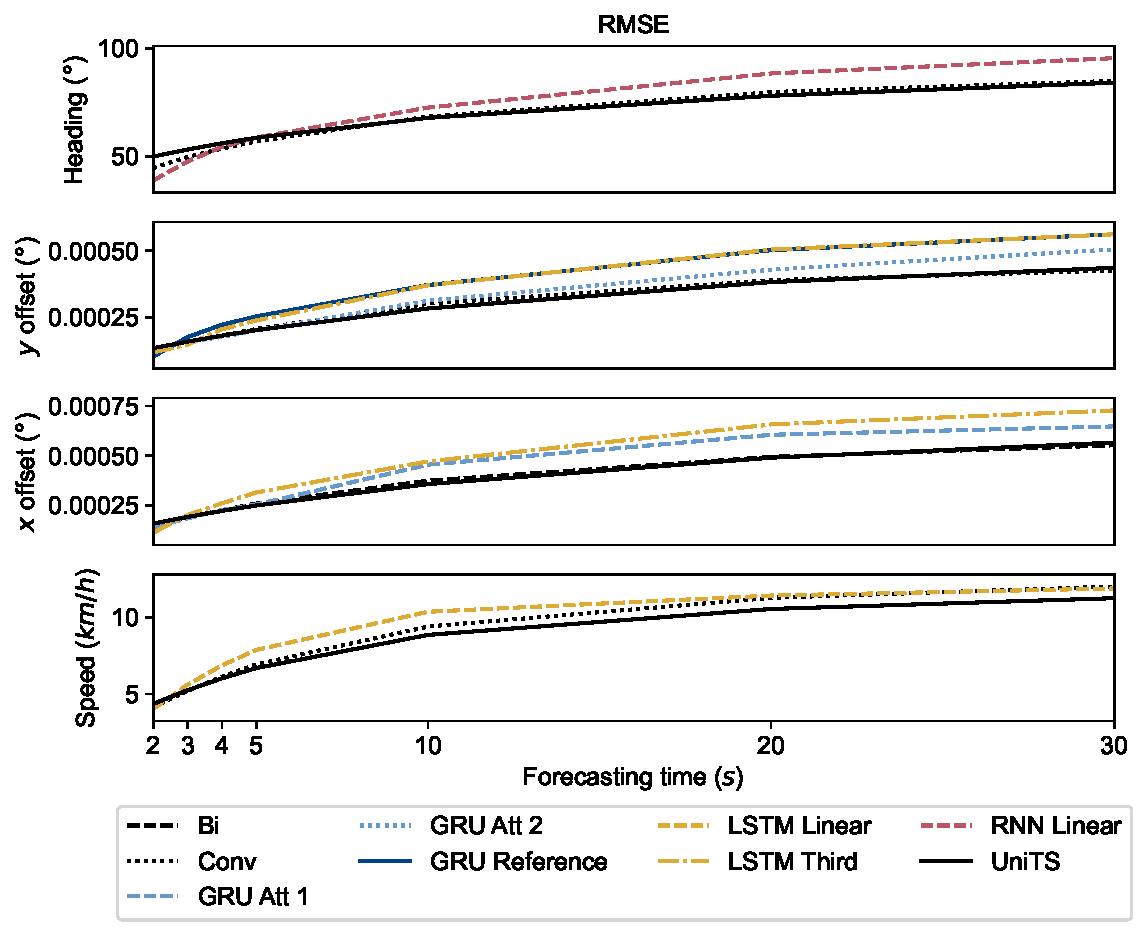
\includegraphics[width = 0.99 \linewidth]{best_RMSE_val_merged.pdf}
	\caption{The average RMSE across $k$-fold testing datasets using different validation datasets for all variables estimated in nested $k$-fold cross-validation by different RNN models, and forecasting times.}
	\label{fig:best_RMSE_val_merged}
\end{figure}

The average RMSE in $\degree$, with standard deviation in brackets, across $k$-fold validation datasets for the heading estimated on the $k$-fold testing datasets by different RNN models, and forecasting times is listed in Table~\ref{tab:best_direction_RMSE}.

\begin{table}[!ht]
	\centering
	\resizebox{\linewidth}{!}{
		\begin{tabular}{|c|c|c|c|c|c|c|c|}
			\hline
			Model & $2$ $s$ & $3$ $s$ & $4$ $s$ & $5$ $s$ & $10$ $s$ & $20$ $s$ & $30$ $s$ \\ \hline
			\multirow{2}{*}{Conv} & $44.62$ & $49.72$ & $\mathbf{53.58}$ & $\mathbf{56.94}$ & $68.41$ & $79.74$ & $84.99$ \\
			 & ($2.02$) & ($2.28$) & \textbf{(}$\mathbf{2.09}$\textbf{)} & \textbf{(}$\mathbf{2.26}$\textbf{)} & ($2.17$) & ($2.29$) & ($2.37$) \\ \hline
			\multirow{2}{*}{RNN Linear} & $\mathbf{38.85}$ & $\mathbf{47.63}$ & $54.36$ & $58.71$ & $72.54$ & $88.35$ & $95.47$ \\
			 & \textbf{(}$\mathbf{1.85}$\textbf{)} & \textbf{(}$\mathbf{2.42}$\textbf{)} & ($2.22$) & ($2.05$) & ($2.33$) & ($1.93$) & ($2.48$) \\ \hline
			\multirow{2}{*}{UniTS} & $49.88$ & $53.14$ & $56.02$ & $58.6$ & $\mathbf{67.8}$ & $\mathbf{78.04}$ & $\mathbf{84.09}$ \\
			 & ($2.18$) & ($2.29$) & ($2.35$) & ($2.38$) & \textbf{(}$\mathbf{2.26}$\textbf{)} & \textbf{(}$\mathbf{2.29}$\textbf{)} & \textbf{(}$\mathbf{2.47}$\textbf{)} \\ \hline
		\end{tabular}
	}
	\caption{The average RMSE in $\degree$, with standard deviation in brackets, across $k$-fold validation datasets for the heading estimated on the $k$-fold testing datasets by different RNN models, and forecasting times.}
	\label{tab:best_direction_RMSE}
\end{table}

The RNN Linear model achieved the lowest RMSE for heading, and a forecasting time of $2$, and $3$ $s$ with average values and standard deviation (in brackets) that equal $38.85$ $\degree$ ($1.85$ $\degree$), and $47.63$ $\degree$ ($2.42$ $\degree$) respectively.

The RNN Linear model does not have a statistically significantly different RMSE than the GRU Linear model for heading using a forecasting time of $2$ $s$, with a $p$-value equaling $3.764 \times 10^{-4}$.

The RNN Linear model does not have a statistically significantly different RMSE than the Conv model for heading using a forecasting time of $3$ $s$, with a $p$-value equaling $8.069 \times 10^{-3}$.

The Conv model achieved the lowest RMSE for heading, and a forecasting time of $4$, and $5$ $s$ with average values and standard deviation (in brackets) that equal $53.58$ $\degree$ ($2.09$ $\degree$), and $56.94$ $\degree$ ($2.26$ $\degree$) respectively.

The Conv model does not have a statistically significantly different RMSE than the GRU Linear, LSTM Linear, RNN Linear, and UniTS models for heading using a forecasting time of $4$ $s$, with $p$-values equaling $1.051 \times 10^{-2}$, $9.635 \times 10^{-3}$, $1.817 \times 10^{-1}$, and $1.155 \times 10^{-3}$.

The Conv model does not have a statistically significantly different RMSE than the GRU Linear, LSTM Linear, RNN Linear, and UniTS models for heading using a forecasting time of $5$ $s$, with $p$-values equaling $1.296 \times 10^{-3}$, $8.081 \times 10^{-4}$, $7.371 \times 10^{-3}$, and $2.551 \times 10^{-2}$.

The UniTS model achieved the lowest RMSE for heading, and a forecasting time of $10$, $20$, and $30$ $s$ with average values and standard deviation (in brackets) that equal $67.8$ $\degree$ ($2.26$ $\degree$), $78.04$ $\degree$ ($2.29$ $\degree$), and $84.09$ $\degree$ ($2.47$ $\degree$) respectively.

The UniTS model does not have a statistically significantly different RMSE than the Bi, and Conv models for heading using a forecasting time of $10$ $s$, with $p$-values equaling $6.263 \times 10^{-2}$, and $3.666 \times 10^{-1}$.

The UniTS model does not have a statistically significantly different RMSE than the Bi, and Conv models for heading using a forecasting time of $20$ $s$, with $p$-values equaling $3.419 \times 10^{-3}$, and $2.191 \times 10^{-2}$.

The UniTS model does not have a statistically significantly different RMSE than the Bi, and Conv models for heading using a forecasting time of $30$ $s$, with $p$-values equaling $1.355 \times 10^{-2}$, and $1.73 \times 10^{-1}$.

\subsection{Results for $y$ Offset}
%\label{subsec:latitude_no_abs_results}
%\vspace{10pt}

The average RMSE in $\degree$ ($\times 10^{-4}$), with standard deviation in brackets, across $k$-fold validation datasets for the $y$ offset estimated on the $k$-fold testing datasets by different RNN models, and forecasting times is listed in Table~\ref{tab:best_latitude_no_abs_RMSE}.

\begin{table}[!ht]
	\centering
	\resizebox{\linewidth}{!}{
		\begin{tabular}{|c|c|c|c|c|c|c|c|}
			\hline
			Model & $2$ $s$ & $3$ $s$ & $4$ $s$ & $5$ $s$ & $10$ $s$ & $20$ $s$ & $30$ $s$ \\ \hline
			\multirow{2}{*}{Conv} & $1.267$ & $1.545$ & $1.817$ & $2.062$ & $3.013$ & $3.894$ & $\mathbf{4.256}$ \\
			 & ($0.136$) & ($0.141$) & ($0.141$) & ($0.156$) & ($0.203$) & ($0.253$) & \textbf{(}$\mathbf{0.257}$\textbf{)} \\ \hline
			\multirow{2}{*}{GRU Att 2} & $1.302$ & $1.584$ & $\mathbf{1.76}$ & $\mathbf{2.007}$ & $3.125$ & $4.289$ & $5.054$ \\
			 & ($0.207$) & ($0.238$) & \textbf{(}$\mathbf{0.198}$\textbf{)} & \textbf{(}$\mathbf{0.213}$\textbf{)} & ($0.26$) & ($0.325$) & ($0.438$) \\ \hline
			\multirow{2}{*}{GRU Reference} & $\mathbf{1.027}$ & $1.757$ & $2.219$ & $2.533$ & $3.711$ & $5.019$ & $5.615$ \\
			 & \textbf{(}$\mathbf{0.266}$\textbf{)} & ($0.357$) & ($0.352$) & ($0.251$) & ($0.276$) & ($0.34$) & ($0.395$) \\ \hline
			\multirow{2}{*}{LSTM Third} & $1.189$ & $\mathbf{1.473}$ & $2.049$ & $2.383$ & $3.701$ & $5.04$ & $5.616$ \\
			 & ($0.346$) & \textbf{(}$\mathbf{0.36}$\textbf{)} & ($0.479$) & ($0.349$) & ($0.23$) & ($0.386$) & ($0.406$) \\ \hline
			\multirow{2}{*}{UniTS} & $1.343$ & $1.586$ & $1.811$ & $2.017$ & $\mathbf{2.831}$ & $\mathbf{3.821}$ & $4.357$ \\
			 & ($0.248$) & ($0.217$) & ($0.21$) & ($0.21$) & \textbf{(}$\mathbf{0.238}$\textbf{)} & \textbf{(}$\mathbf{0.301}$\textbf{)} & ($0.331$) \\ \hline
		\end{tabular}
	}
	\caption{The average RMSE in $\degree$ ($\times 10^{-4}$), with standard deviation in brackets, across $k$-fold validation datasets for the $y$ offset estimated on the $k$-fold testing datasets by different RNN models, and forecasting times.}
	\label{tab:best_latitude_no_abs_RMSE}
\end{table}

The GRU Reference model achieved the lowest RMSE for $y$ offset, and a forecasting time of $2$ $s$ with an average value and standard deviation (in brackets) that equals $10.265 \times 10^{-5}$ $\degree$ ($2.66 \times 10^{-5}$ $\degree$).

The GRU Reference model does not have a statistically significantly different RMSE than the Conv, GRU Att 1, GRU Linear, GRU Third, GRU Twice, LSTM Linear, LSTM Reference, and LSTM Third models for $y$ offset using a forecasting time of $2$ $s$, with $p$-values equaling $1.453 \times 10^{-3}$, $3.781 \times 10^{-3}$, $1.908 \times 10^{-1}$, $9.573 \times 10^{-2}$, $6.338 \times 10^{-1}$, $3.419 \times 10^{-3}$, $1.485 \times 10^{-1}$, and $9.032 \times 10^{-2}$.

The LSTM Third model achieved the lowest RMSE for $y$ offset, and a forecasting time of $3$ $s$ with an average value and standard deviation (in brackets) that equals $14.733 \times 10^{-5}$ $\degree$ ($3.604 \times 10^{-5}$ $\degree$).

The LSTM Third model does not have a statistically significantly different RMSE than the Bi, Conv, GRU Att 1, GRU Att 2, GRU Att 3, GRU Att 4, GRU Linear, GRU Reference, GRU Third, GRU Twice, LSTM Linear, LSTM Reference, and UniTS models for $y$ offset using a forecasting time of $3$ $s$, with $p$-values equaling $2.025 \times 10^{-3}$, $1.908 \times 10^{-1}$, $1.874 \times 10^{-2}$, $2.748 \times 10^{-2}$, $4.895 \times 10^{-4}$, $3.088 \times 10^{-3}$, $5.072 \times 10^{-3}$, $1.027 \times 10^{-3}$, $9.032 \times 10^{-2}$, $6.721 \times 10^{-1}$, $2.191 \times 10^{-2}$, $4.605 \times 10^{-3}$, and $8.822 \times 10^{-3}$.

The GRU Att 2 model achieved the lowest RMSE for $y$ offset, and a forecasting time of $4$, and $5$ $s$ with average values and standard deviation (in brackets) that equal $17.603 \times 10^{-5}$ $\degree$ ($1.979 \times 10^{-5}$ $\degree$), and $20.067 \times 10^{-5}$ $\degree$ ($2.131 \times 10^{-5}$ $\degree$) respectively.

The GRU Att 2 model does not have a statistically significantly different RMSE than the Bi, Conv, GRU Att 1, LSTM Third, LSTM Twice, and UniTS models for $y$ offset using a forecasting time of $4$ $s$, with $p$-values equaling $1.625 \times 10^{-3}$, $2.304 \times 10^{-1}$, $2.551 \times 10^{-2}$, $4.605 \times 10^{-3}$, $1.453 \times 10^{-3}$, and $6.129 \times 10^{-3}$.

The GRU Att 2 model does not have a statistically significantly different RMSE than the Bi, Conv, GRU Att 1, and UniTS models for $y$ offset using a forecasting time of $5$ $s$, with $p$-values equaling $6.129 \times 10^{-3}$, and $3.525 \times 10^{-1}$, $1.355 \times 10^{-2}$, and $3.525 \times 10^{-1}$.

The UniTS model achieved the lowest RMSE for $y$ offset, and a forecasting time of $10$, and $20$ $s$ with average values and standard deviation (in brackets) that equal $28.309 \times 10^{-5}$ $\degree$ ($2.382 \times 10^{-5}$ $\degree$), and $38.21 \times 10^{-5}$ $\degree$ ($3.005 \times 10^{-5}$ $\degree$) respectively.

The UniTS model does not have a statistically significantly different RMSE than the Bi, and Conv models for $y$ offset using a forecasting time of $10$ $s$, with $p$-values equaling $3.781 \times 10^{-3}$, and $1.145 \times 10^{-2}$.

The UniTS model does not have a statistically significantly different RMSE than the Bi, and Conv models for $y$ offset using a forecasting time of $20$ $s$, with $p$-values equaling $2.411 \times 10^{-1}$, and $3.123 \times 10^{-1}$.

The Conv model achieved the lowest RMSE for $y$ offset, and a forecasting time of $30$ $s$ with an average value and standard deviation (in brackets) that equals $42.559 \times 10^{-5}$ $\degree$ ($2.572 \times 10^{-5}$ $\degree$).

The Conv model does not have a statistically significantly different RMSE than the UniTS model for $y$ offset using a forecasting time of $30$ $s$, with a $p$-value equaling $2.872 \times 10^{-1}$.

\subsection{Results for $x$ Offset}
%\label{subsec:longitude_no_abs_results}
%\vspace{10pt}

The average RMSE in $\degree$ ($\times 10^{-4}$), with standard deviation in brackets, across $k$-fold validation datasets for the $x$ offset estimated on the $k$-fold testing datasets by different RNN models, and forecasting times is listed in Table~\ref{tab:best_longitude_no_abs_RMSE}.

\begin{table}[!ht]
	\centering
	\resizebox{\linewidth}{!}{
		\begin{tabular}{|c|c|c|c|c|c|c|c|}
			\hline
			Model & $2$ $s$ & $3$ $s$ & $4$ $s$ & $5$ $s$ & $10$ $s$ & $20$ $s$ & $30$ $s$ \\ \hline
			\multirow{2}{*}{Bi} & $1.512$ & $1.903$ & $2.257$ & $2.589$ & $3.74$ & $4.936$ & $\mathbf{5.52}$ \\
			 & ($0.154$) & ($0.196$) & ($0.231$) & ($0.257$) & ($0.327$) & ($0.333$) & \textbf{(}$\mathbf{0.397}$\textbf{)} \\ \hline
			\multirow{2}{*}{GRU Att 1} & $1.401$ & $\mathbf{1.846}$ & $2.265$ & $2.541$ & $4.544$ & $6.046$ & $6.47$ \\
			 & ($0.188$) & \textbf{(}$\mathbf{0.24}$\textbf{)} & ($0.271$) & ($0.274$) & ($0.694$) & ($0.471$) & ($0.597$) \\ \hline
			\multirow{2}{*}{LSTM Third} & $\mathbf{1.123}$ & $2.014$ & $2.601$ & $3.145$ & $4.704$ & $6.568$ & $7.272$ \\
			 & \textbf{(}$\mathbf{0.201}$\textbf{)} & ($0.379$) & ($0.368$) & ($0.363$) & ($0.408$) & ($0.475$) & ($0.428$) \\ \hline
			\multirow{2}{*}{UniTS} & $1.582$ & $1.917$ & $\mathbf{2.219}$ & $\mathbf{2.494}$ & $\mathbf{3.565}$ & $\mathbf{4.895}$ & $5.654$ \\
			 & ($0.178$) & ($0.202$) & \textbf{(}$\mathbf{0.224}$\textbf{)} & \textbf{(}$\mathbf{0.244}$\textbf{)} & \textbf{(}$\mathbf{0.319}$\textbf{)} & \textbf{(}$\mathbf{0.404}$\textbf{)} & ($0.433$) \\ \hline
		\end{tabular}
	}
	\caption{The average RMSE in $\degree$ ($\times 10^{-4}$), with standard deviation in brackets, across $k$-fold validation datasets for the $x$ offset estimated on the $k$-fold testing datasets by different RNN models, and forecasting times.}
	\label{tab:best_longitude_no_abs_RMSE}
\end{table}

The LSTM Third model achieved the lowest RMSE for $x$ offset, and a forecasting time of $2$ $s$ with an average value and standard deviation (in brackets) that equals $11.23 \times 10^{-5}$ $\degree$ ($2.01 \times 10^{-5}$ $\degree$).

The LSTM Third model does not have a statistically significantly different RMSE than the GRU Linear, GRU Third, GRU Twice, LSTM Linear, and LSTM Reference models for $x$ offset using a forecasting time of $2$ $s$, with $p$-values equaling $6.313 \times 10^{-4}$, $7.112 \times 10^{-1}$, $5.424 \times 10^{-1}$, $6.263 \times 10^{-2}$, and $2.027 \times 10^{-2}$.

The GRU Att 1 model achieved the lowest RMSE for $x$ offset, and a forecasting time of $3$ $s$ with an average value and standard deviation (in brackets) that equals $18.46 \times 10^{-5}$ $\degree$ ($2.4 \times 10^{-5}$ $\degree$).

The GRU Att 1 model does not have a statistically significantly different RMSE than the Bi, Conv, GRU Att 2, GRU Third, GRU Twice, LSTM Linear, LSTM Third, LSTM Twice, RNN Third, and UniTS models for $x$ offset using a forecasting time of $3$ $s$, with $p$-values equaling $3.254 \times 10^{-1}$, $6.721 \times 10^{-1}$, $1.073 \times 10^{-1}$, $2.255 \times 10^{-3}$, $4.605 \times 10^{-3}$, $5.564 \times 10^{-4}$, $2.027 \times 10^{-2}$, $9.789 \times 10^{-1}$, $3.764 \times 10^{-4}$, and $7.15 \times 10^{-4}$.

The UniTS model achieved the lowest RMSE for $x$ offset, and a forecasting time of $4$, $5$, $10$, and $20$ $s$ with average values and standard deviation (in brackets) that equal $22.19 \times 10^{-5}$ $\degree$ ($2.24 \times 10^{-5}$ $\degree$), $24.94 \times 10^{-5}$ $\degree$ ($2.44 \times 10^{-5}$ $\degree$), $35.65 \times 10^{-5}$ $\degree$ ($3.19 \times 10^{-5}$ $\degree$), and $48.95 \times 10^{-5}$ $\degree$ ($4.04 \times 10^{-5}$ $\degree$) respectively.

The UniTS model does not have a statistically significantly different RMSE than the Bi, Conv, GRU Att 1, GRU Att 2, and GRU Att 3 models for $x$ offset using a forecasting time of $4$ $s$, with $p$-values equaling $5.965 \times 10^{-1}$, $2.411 \times 10^{-1}$, $5.875 \times 10^{-2}$, $1.908 \times 10^{-1}$, and $3.291 \times 10^{-4}$.

The UniTS model does not have a statistically significantly different RMSE than the Bi, Conv, GRU Att 1, and GRU Att 2 models for $x$ offset using a forecasting time of $5$ $s$, with $p$-values equaling $9.032 \times 10^{-2}$, $3.291 \times 10^{-4}$, $2.748 \times 10^{-2}$, and $9.032 \times 10^{-2}$.

The UniTS model does not have a statistically significantly different RMSE than the Bi model for $x$ offset using a forecasting time of $10$ $s$, with a $p$-value equaling $6.263 \times 10^{-2}$.

The UniTS model does not have a statistically significantly different RMSE than the Bi model for $x$ offset using a forecasting time of $20$ $s$, with a $p$-value equaling $7.712 \times 10^{-1}$.

The Bi model achieved the lowest RMSE for $x$ offset, and a forecasting time of $30$ $s$ with an average value and standard deviation (in brackets) that equals $55.2 \times 10^{-5}$ $\degree$ ($3.97 \times 10^{-5}$ $\degree$).

The Bi model does not have a statistically significantly different RMSE than the UniTS model for $x$ offset using a forecasting time of $30$ $s$, with a $p$-value equaling $2.996 \times 10^{-1}$.

\subsection{Results for Speed}
%\label{subsec:speed_results}
%\vspace{10pt}

The average RMSE in $km/h$, with standard deviation in brackets, across $k$-fold validation datasets for the speed estimated on the $k$-fold testing datasets by different RNN models, and forecasting times is listed in Table~\ref{tab:best_speed_RMSE}.

\begin{table}[!ht]
	\centering
	\resizebox{\linewidth}{!}{
		\begin{tabular}{|c|c|c|c|c|c|c|c|}
			\hline
			Model & $2$ $s$ & $3$ $s$ & $4$ $s$ & $5$ $s$ & $10$ $s$ & $20$ $s$ & $30$ $s$ \\ \hline
			\multirow{2}{*}{Conv} & $4.16$ & $\mathbf{5.2}$ & $6.12$ & $6.93$ & $9.41$ & $11.29$ & $12.02$ \\
			 & ($0.3$) & \textbf{(}$\mathbf{0.37}$\textbf{)} & ($0.43$) & ($0.48$) & ($0.64$) & ($0.7$) & ($0.71$) \\ \hline
			\multirow{2}{*}{LSTM Linear} & $\mathbf{4.03}$ & $5.61$ & $6.87$ & $7.88$ & $10.37$ & $11.43$ & $11.9$ \\
			 & \textbf{(}$\mathbf{0.3}$\textbf{)} & ($0.45$) & ($0.53$) & ($0.59$) & ($0.71$) & ($0.75$) & ($0.76$) \\ \hline
			\multirow{2}{*}{UniTS} & $4.35$ & $5.25$ & $\mathbf{6.02}$ & $\mathbf{6.69}$ & $\mathbf{8.86}$ & $\mathbf{10.55}$ & $\mathbf{11.26}$ \\
			 & ($0.3$) & ($0.37$) & \textbf{(}$\mathbf{0.42}$\textbf{)} & \textbf{(}$\mathbf{0.47}$\textbf{)} & \textbf{(}$\mathbf{0.64}$\textbf{)} & \textbf{(}$\mathbf{0.77}$\textbf{)} & \textbf{(}$\mathbf{0.75}$\textbf{)} \\ \hline
		\end{tabular}
	}
	\caption{The average RMSE in $km/h$, with standard deviation in brackets, across $k$-fold validation datasets for the speed estimated on the $k$-fold testing datasets by different RNN models, and forecasting times.}
	\label{tab:best_speed_RMSE}
\end{table}

The LSTM Linear model achieved the lowest RMSE for speed, and a forecasting time of $2$ $s$ with an average value and standard deviation (in brackets) that equals $4.03$ $km/h$ ($0.3$ $km/h$).

The LSTM Linear model does not have a statistically significantly different RMSE than the Bi, Conv, GRU Linear, and RNN Linear models for speed using a forecasting time of $2$ $s$, with $p$-values equaling $1.266 \times 10^{-1}$, $1.645 \times 10^{-1}$, $2.099 \times 10^{-1}$, and $2.002 \times 10^{-1}$.

The Conv model achieved the lowest RMSE for speed, and a forecasting time of $3$ $s$ with an average value and standard deviation (in brackets) that equals $5.2$ $km/h$ ($0.37$ $km/h$).

The Conv model does not have a statistically significantly different RMSE than the GRU Linear, LSTM Linear, RNN Linear, and UniTS models for speed using a forecasting time of $3$ $s$, with $p$-values equaling $1.027 \times 10^{-3}$, $2.255 \times 10^{-3}$, $3.419 \times 10^{-3}$, and $4.742 \times 10^{-1}$.

The UniTS model achieved the lowest RMSE for speed, and a forecasting time of $4$, $5$, $10$, $20$, and $30$ $s$ with average values and standard deviation (in brackets) that equal $6.02$ $km/h$ ($0.42$ $km/h$), $6.69$ $km/h$ ($0.47$ $km/h$), $8.86$ $km/h$ ($0.64$ $km/h$), $10.55$ $km/h$ ($0.77$ $km/h$), and $11.26$ $km/h$ ($0.75$ $km/h$) respectively.

The UniTS model does not have a statistically significantly different RMSE than the Bi, and Conv models for speed using a forecasting time of $4$ $s$, with $p$-values equaling $1.908 \times 10^{-1}$, and $3.81 \times 10^{-1}$.

The UniTS model does not have a statistically significantly different RMSE than the Bi, and Conv models for speed using a forecasting time of $5$ $s$, with $p$-values equaling $4.826 \times 10^{-2}$, and $1.336 \times 10^{-1}$.

The UniTS model does not have a statistically significantly different RMSE than the Bi, and Conv models for speed using a forecasting time of $10$ $s$, with $p$-values equaling $2.785 \times 10^{-3}$, and $7.371 \times 10^{-3}$.

The UniTS model does not have a statistically significantly different RMSE than the Bi, and Conv models for speed using a forecasting time of $20$ $s$, with $p$-values equaling $9.119 \times 10^{-4}$, and $2.255 \times 10^{-3}$.

The UniTS model does not have a statistically significantly different RMSE than the Bi, and Conv models for speed using a forecasting time of $30$ $s$, with $p$-values equaling $8.081 \times 10^{-4}$, and $1.453 \times 10^{-3}$.

\subsection{Results for Trajectories Estimated Using $x$ and $y$ Offset}
%\label{subsec:no_abs_results}
%\vspace{10pt}

Figure~\ref{fig:best_RMSE_traj_val_merged} contains the average RMSE across $k$-fold testing datasets using different trajectory estimation methods, validation datasets for all trajectories estimated in nested $k$-fold cross-validation by different trajectory estimation methods, RNN models, and forecasting times.

\begin{figure}[!ht]
	\centering
	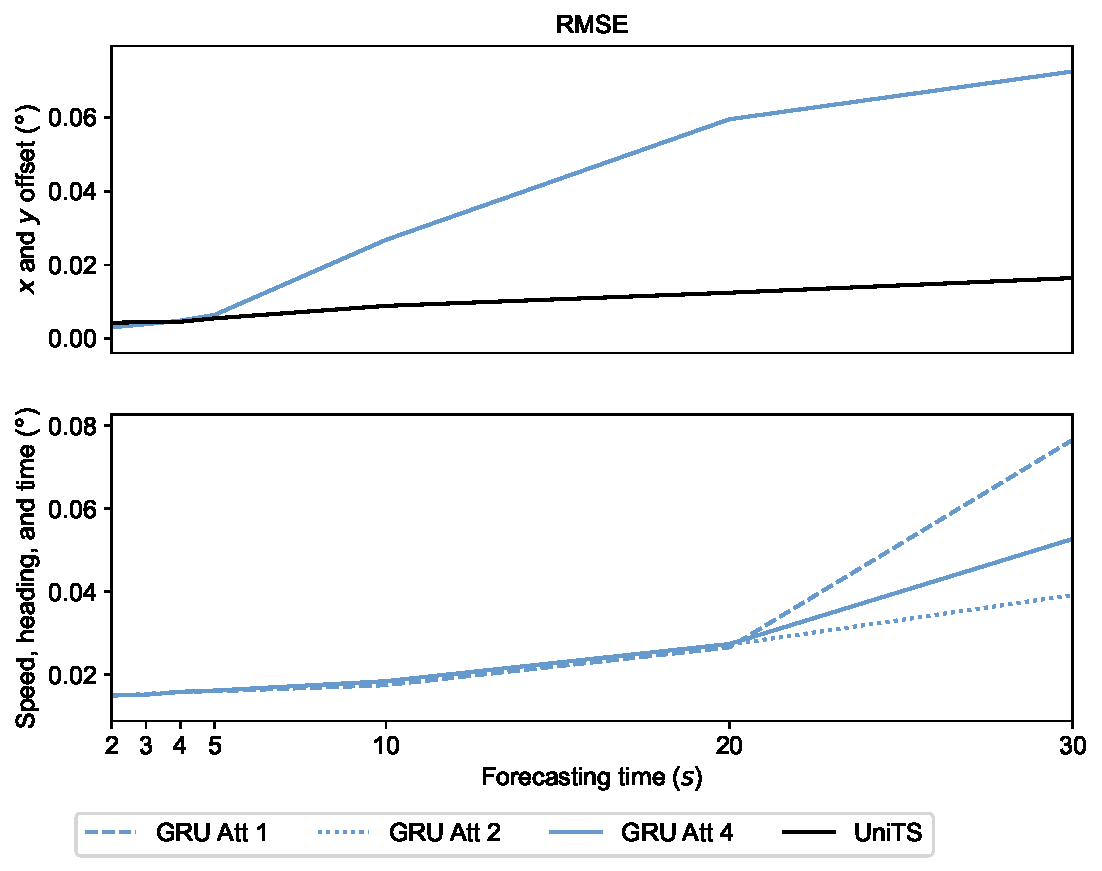
\includegraphics[width = 0.99 \linewidth]{best_RMSE_traj_val_merged.pdf}
	\caption{The average RMSE across $k$-fold testing datasets using different trajectory estimation methods, validation datasets for all trajectories estimated in nested $k$-fold cross-validation by different trajectory estimation methods, RNN models, and forecasting times.}
	\label{fig:best_RMSE_traj_val_merged}
\end{figure}

The average RMSE in $\degree$ ($\times 10^{-3}$), with standard deviation in brackets, across $k$-fold validation datasets for the trajectories in the $k$-fold testing datasets estimated using $x$ and $y$ offset, different RNN models, and forecasting times is listed in Table~\ref{tab:best_no_abs_RMSE}.

\begin{table}[!ht]
	\centering
	\resizebox{\linewidth}{!}{
		\begin{tabular}{|c|c|c|c|c|c|c|c|}
			\hline
			Model & $2$ $s$ & $3$ $s$ & $4$ $s$ & $5$ $s$ & $10$ $s$ & $20$ $s$ & $30$ $s$ \\ \hline
			\multirow{2}{*}{GRU Att 4} & $\mathbf{3.05}$ & $\mathbf{3.86}$ & $4.86$ & $6.4$ & $26.8$ & $59.52$ & $72.49$ \\
			 & \textbf{(}$\mathbf{0.49}$\textbf{)} & \textbf{(}$\mathbf{0.51}$\textbf{)} & ($0.52$) & ($0.85$) & ($6.96$) & ($9.83$) & ($19.4$) \\ \hline
			\multirow{2}{*}{UniTS} & $4.26$ & $4.47$ & $\mathbf{4.54}$ & $\mathbf{5.47}$ & $\mathbf{8.86}$ & $\mathbf{12.43}$ & $\mathbf{16.41}$ \\
			 & ($3.51$) & ($2.91$) & \textbf{(}$\mathbf{0.66}$\textbf{)} & \textbf{(}$\mathbf{0.97}$\textbf{)} & \textbf{(}$\mathbf{1.37}$\textbf{)} & \textbf{(}$\mathbf{1.55}$\textbf{)} & \textbf{(}$\mathbf{2.47}$\textbf{)} \\ \hline
		\end{tabular}
	}
	\caption{The average RMSE in $\degree$ ($\times 10^{-3}$), with standard deviation in brackets, across $k$-fold validation datasets for the trajectories in the $k$-fold testing datasets estimated using $x$ and $y$ offset, different RNN models, and forecasting times.}
	\label{tab:best_no_abs_RMSE}
\end{table}

The GRU Att 4 model achieved the lowest RMSE for trajectories estimated using $x$ and $y$ offset, and a forecasting time of $2$, and $3$ $s$ with average values and standard deviation (in brackets) that equal $3.05 \times 10^{-3}$ $\degree$ ($0.49 \times 10^{-3}$ $\degree$), and $3.86 \times 10^{-3}$ $\degree$ ($0.51 \times 10^{-3}$ $\degree$) respectively.

The GRU Att 4 model does not have a statistically significantly different RMSE than the GRU Att 1, GRU Att 3, and UniTS models for trajectories estimated using $x$ and $y$ offset, and a forecasting time of $2$ $s$, with $p$-values equaling $5.579 \times 10^{-3}$, $7.098 \times 10^{-2}$, and $9.119 \times 10^{-4}$.

The GRU Att 4 model does not have a statistically significantly different RMSE than the GRU Att 1, and UniTS models for trajectories estimated using $x$ and $y$ offset, and a forecasting time of $3$ $s$, with $p$-values equaling $3.417 \times 10^{-2}$, and $5.077 \times 10^{-1}$.

The UniTS model achieved the lowest RMSE for trajectories estimated using $x$ and $y$ offset, and a forecasting time of $4$, $5$, $10$, $20$, and $30$ $s$ with average values and standard deviation (in brackets) that equal $4.54 \times 10^{-3}$ $\degree$ ($0.66 \times 10^{-3}$ $\degree$), $5.47 \times 10^{-3}$ $\degree$ ($0.97 \times 10^{-3}$ $\degree$), $8.86 \times 10^{-3}$ $\degree$ ($1.37 \times 10^{-3}$ $\degree$), $12.43 \times 10^{-3}$ $\degree$ ($1.55 \times 10^{-3}$ $\degree$), and $16.41 \times 10^{-3}$ $\degree$ ($2.47 \times 10^{-3}$ $\degree$) respectively.

The UniTS model does not have a statistically significantly different RMSE than the GRU Att 1, and GRU Att 4 models for trajectories estimated using $x$ and $y$ offset, and a forecasting time of $4$ $s$, with $p$-values equaling $4.297 \times 10^{-4}$, and $5.158 \times 10^{-2}$.

The UniTS model does not have a statistically significantly different RMSE than the GRU Att 4 model for trajectories estimated using $x$ and $y$ offset, and a forecasting time of $5$ $s$, with a $p$-value equaling $1.027 \times 10^{-3}$.

\subsection{Results for Trajectories Estimated Using Speed, Heading, and Time}
%\label{subsec:speed_actual_dir_results}
%\vspace{10pt}

The average RMSE in $\degree$ ($\times 10^{-2}$), with standard deviation in brackets, across $k$-fold validation datasets for the trajectories in the $k$-fold testing datasets estimated using speed, heading, and time, different RNN models, and forecasting times is listed in Table~\ref{tab:best_speed_actual_dir_RMSE}.

\begin{table}[!ht]
	\centering
	\resizebox{\linewidth}{!}{
		\begin{tabular}{|c|c|c|c|c|c|c|c|}
			\hline
			Model & $2$ $s$ & $3$ $s$ & $4$ $s$ & $5$ $s$ & $10$ $s$ & $20$ $s$ & $30$ $s$ \\ \hline
			\multirow{2}{*}{GRU Att 1} & $1.501$ & $1.524$ & $1.587$ & $\mathbf{1.598}$ & $\mathbf{1.745}$ & $\mathbf{2.657}$ & $7.659$ \\
			 & ($0.163$) & ($0.154$) & ($0.163$) & \textbf{(}$\mathbf{0.135}$\textbf{)} & \textbf{(}$\mathbf{0.108}$\textbf{)} & \textbf{(}$\mathbf{0.17}$\textbf{)} & ($6.196$) \\ \hline
			\multirow{2}{*}{GRU Att 2} & $1.495$ & $1.536$ & $1.586$ & $1.616$ & $1.818$ & $2.72$ & $\mathbf{3.919}$ \\
			 & ($0.161$) & ($0.177$) & ($0.173$) & ($0.165$) & ($0.192$) & ($0.19$) & \textbf{(}$\mathbf{0.589}$\textbf{)} \\ \hline
			\multirow{2}{*}{GRU Att 4} & $\mathbf{1.494}$ & $\mathbf{1.514}$ & $\mathbf{1.581}$ & $1.616$ & $1.842$ & $2.737$ & $5.269$ \\
			 & \textbf{(}$\mathbf{0.152}$\textbf{)} & \textbf{(}$\mathbf{0.163}$\textbf{)} & \textbf{(}$\mathbf{0.173}$\textbf{)} & ($0.15$) & ($0.125$) & ($0.238$) & ($4.403$) \\ \hline
		\end{tabular}
	}
	\caption{The average RMSE in $\degree$ ($\times 10^{-2}$), with standard deviation in brackets, across $k$-fold validation datasets for the trajectories in the $k$-fold testing datasets estimated using speed, heading, and time, different RNN models, and forecasting times.}
	\label{tab:best_speed_actual_dir_RMSE}
\end{table}

The GRU Att 4 model achieved the lowest RMSE for trajectories estimated using speed, heading, and time, and a forecasting time of $2$, $3$, and $4$ $s$ with average values and standard deviation (in brackets) that equal $14.94 \times 10^{-3}$ $\degree$ ($1.52 \times 10^{-3}$ $\degree$), $15.14 \times 10^{-3}$ $\degree$ ($1.63 \times 10^{-3}$ $\degree$), and $15.81 \times 10^{-3}$ $\degree$ ($1.73 \times 10^{-3}$ $\degree$) respectively.

The GRU Att 4 model does not have a statistically significantly different RMSE than the GRU Att 1, GRU Att 2, and GRU Att 3 models for trajectories estimated using speed, heading, and time, and a forecasting time of $2$ $s$, with $p$-values equaling $3.81 \times 10^{-1}$, $5.249 \times 10^{-1}$, and $2.027 \times 10^{-2}$.

The GRU Att 4 model does not have a statistically significantly different RMSE than the GRU Att 1, GRU Att 2, and GRU Att 3 models for trajectories estimated using speed, heading, and time, and a forecasting time of $3$ $s$, with $p$-values equaling $4.108 \times 10^{-1}$, $2.872 \times 10^{-1}$, and $2.027 \times 10^{-2}$.

The GRU Att 4 model does not have a statistically significantly different RMSE than the GRU Att 1, GRU Att 2, and GRU Att 3 models for trajectories estimated using speed, heading, and time, and a forecasting time of $4$ $s$, with $p$-values equaling $6.528 \times 10^{-1}$, $9.578 \times 10^{-1}$, and $5.875 \times 10^{-2}$.

The GRU Att 1 model achieved the lowest RMSE for trajectories estimated using speed, heading, and time, and a forecasting time of $5$, $10$, and $20$ $s$,  with average values and standard deviation (in brackets) that equal $15.98 \times 10^{-3}$ $\degree$ ($1.35 \times 10^{-3}$ $\degree$), $17.45 \times 10^{-3}$ $\degree$ ($1.08 \times 10^{-3}$ $\degree$), and $26.57 \times 10^{-3}$ $\degree$ ($1.7 \times 10^{-3}$ $\degree$) respectively.

The GRU Att 1 model does not have a statistically significantly different RMSE than the GRU Att 2 model for trajectories estimated using speed, heading, and time, and a forecasting time of $10$ $s$, with a $p$-value equaling $1.874 \times 10^{-2}$.

The GRU Att 1 model does not have a statistically significantly different RMSE than the GRU Att 2, GRU Att 3, and GRU Att 4 models for trajectories estimated using speed, heading, and time, and a forecasting time of $20$ $s$, with $p$-values equaling $4.215 \times 10^{-2}$, $7.15 \times 10^{-4}$, and $8.069 \times 10^{-3}$.

The GRU Att 1 model does not have a statistically significantly different RMSE than the GRU Att 2, GRU Att 3, and GRU Att 4 models for trajectories estimated using speed, heading, and time, and a forecasting time of $5$ $s$, with $p$-values equaling $7.712 \times 10^{-1}$, $1.73 \times 10^{-1}$, and $1.485 \times 10^{-1}$.

The GRU Att 2 model achieved the lowest RMSE for trajectories estimated using speed, heading, and time, and a forecasting time of $30$ $s$ with an average value and standard deviation (in brackets) that equals $39.19 \times 10^{-3}$ $\degree$ ($5.89 \times 10^{-3}$ $\degree$).

The GRU Att 2 model does not have a statistically significantly different RMSE than the GRU Att 1, GRU Att 3, and GRU Att 4 models for trajectories estimated using speed, heading, and time, and a forecasting time of $30$ $s$, with $p$-values equaling $3.419 \times 10^{-3}$, $7.098 \times 10^{-2}$, and $1.817 \times 10^{-1}$.
 
\subsection{Comparison with State of the Art}

Table~\ref{tab:lateral_position} and Table~\ref{tab:longitudinal_speed} list RMSE values for the most successful state-of-the-art and tested models for $y$ offset and speed. 

Altché and de La Fortelle create a bagged model by averaging the outputs from the four best models. These models are marked by a * in Table~\ref{tab:lateral_position} and Table~\ref{tab:longitudinal_speed}, with bagging almost always performing better than individual models. The study by Altché and de La Fortelle \cite{altche2017lstm} uses LSTM RNN models, while Liu et al. \cite{liu2014vehicle} use a Multi-Layer Perceptron (MLP) without a recurrent layer. 

To compare the results of models from the literature, the $y$ offset values were converted from a range of $0.1$ $\degree$ latitude after preprocessing back to the original range. Values in $\degree$ were then multiplied by $111000$ since $1$ $\degree$ is approximately $111$ $km$ and $1$ $km$ is $1000$ $m$. 

Values of speed in $km/h$ were converted to $m/s$ using the equality $1$ $km/h$ $=$ $1 / 3.6$ $m/s = 0.278$ $m/s$. The only improvement in the tested models was the RMSE value of $2.46$ $m/s$ for speed and a forecasting time of $10$ $s$ with the UniTS model.

\begin{table}[!ht]
	\centering
    \begin{tabular}{|c|c|c|c|c|}
        \hline
        Model & $2$ $s$ & $3$ $s$ & $4$ $s$ & $10$ $s$ \\ \hline
        Reference* & $0.25$ & $\mathbf{0.33}$ & $\mathbf{0.4}$ & $0.73$ \\
        Type* & $0.39$ & $0.44$ & $0.48$ & $0.69$ \\
        No $f$ $f$* & $\mathbf{0.24}$ & $0.33$ & $0.41$ & $0.76$ \\
        No bypass & $0.82$ & $0.85$ & $0.88$ & $1.03$ \\
        Bypass before & $0.38$ & $0.43$ & $0.46$ & $0.68$ \\
        Lin. activ. & $1.39$ & $1.4$ & $1.42$ & $1.56$ \\
        2 LSTMs & $1.26$ & $1.28$ & $1.29$ & $1.41$ \\
        3 dense* & $0.38$ & $0.44$ & $0.5$ & $0.72$ \\
        MLP & $0.32$ & $0.71$ & $/$ & $/$ \\
        Bagged & $0.25$ & $0.33$ & $0.4$ & $\mathbf{0.65}$ \\ \hline
        GRU Att 2 & $1.44$ & $1.76$ & $1.95$ & $3.47$ \\
        GRU Reference & $1.14$ & $1.95$ & $2.46$ & $4.12$ \\
        LSTM Third & $1.32$ & $1.64$ & $2.27$ & $4.11$ \\
        UniTS & $1.49$ & $1.76$ & $2.01$ & $3.14$ \\ \hline
    \end{tabular}
    \caption{RMSE in $m$ for state-of-the-art models from the literature (top) and the tested models (bottom) for $y$ offset.}
    \label{tab:lateral_position}
\end{table}

\begin{table}[!ht]
	\centering
    \begin{tabular}{|c|c|c|c|c|}
        \hline
        Model & $2$ $s$ & $3$ $s$ & $4$ $s$ & $10$ $s$ \\ \hline
        Reference* & $0.99$ & $1.25$ & $1.49$ & $2.96$ \\
        Type* & $0.88$ & $1.05$ & $1.25$ & $2.74$ \\
        No $f$ $f$* & $0.91$ & $1.16$ & $1.44$ & $2.84$ \\
        No bypass & $1.5$ & $1.55$ & $1.66$ & $2.89$ \\
        Bypass before & $0.9$ & $1.06$ & $1.26$ & $2.78$ \\
        Lin. activ. & $1.1$ & $1.34$ & $1.56$ & $2.94$ \\
        2 LSTMs & $1.14$ & $1.42$ & $1.71$ & $3.17$ \\
        3 dense* & $0.87$ & $1.04$ & $1.25$ & $2.77$ \\
        Bagged & $\mathbf{0.81}$ & $\mathbf{0.98}$ & $\mathbf{1.18}$ & $2.48$ \\ \hline
        Conv & $1.16$ & $1.44$ & $1.7$ & $2.61$ \\
        LSTM Linear & $1.12$ & $1.56$ & $1.91$ & $2.88$ \\
        UniTS & $1.21$ & $1.46$ & $1.67$ & $\mathbf{2.46}$ \\ \hline
    \end{tabular}
    \caption{RMSE in $m/s$ for state-of-the-art models from the from the literature (top) and the tested models (bottom) for speed.}
    \label{tab:longitudinal_speed}
\end{table}

\section{Discussion}
\label{sec:Discussion}
%\vspace{10pt}

Table~\ref{tab:best_direction_RMSE}, Table~\ref{tab:best_latitude_no_abs_RMSE}, Table~\ref{tab:best_longitude_no_abs_RMSE}, Table~\ref{tab:best_speed_RMSE}, and Figure~\ref{fig:best_RMSE_val_merged} contain the average RMSE, with standard deviation in brackets, for all variables estimated in nested $k$-fold cross-validation by different RNN models, and forecasting times.

The UniTS model achieved the lowest RMSE for speed and heading forecasting using a forecasting time of $10$, $20$, or $30$ $s$. The UniTS model achieved the lowest RMSE for $x$ and $y$ offset using a forecasting time of $10$, or $20$ $s$. The Bi and Conv model achieved the lowest RMSE using a forecasting time of $30$ $s$, and $x$ and $y$ offset respectively, but they do not have a statistically significantly different average RMSE than the UniTS model for these variables and forecasting time. This proves that the UniTS model should be preferred to the other tested models in future work, especially for long-term forecasting.

The average RMSE for the $y$ offset and the UniTS model increased from $1.343 \times 10^{-4}$ $\degree$ to $4.357 \times 10^{-4}$ $\degree$ when increasing forecasting time from $2$ to $30$ $s$.

The observed decrease in accuracy with larger forecasting times, present for all variables, was expected because errors accumulate. Figure~\ref{fig:2_merge_val} and Figure~\ref{fig:30_merge_val} demonstrate this when comparing trajectories estimated using $x$ and $y$ offset, the UniTS model, and a forecasting time of $2$, and $30$ $s$.

\begin{figure}[!ht]
    \centering
    \includegraphics[width = 0.99 \linewidth]{2_merge_val.pdf}
    \caption{The original black trajectories compared with blue trajectories estimated using $x$ and $y$ offset, the UniTS model, and a forecasting time of $2$ $s$.}
    \label{fig:2_merge_val}
\end{figure}

\begin{figure}[!ht]
    \centering
    \includegraphics[width = 0.99 \linewidth]{30_merge_val.pdf}
    \caption{The original black trajectories compared with blue trajectories estimated using $x$ and $y$ offset, the UniTS model, and a forecasting time of $30$ $s$.}
    \label{fig:30_merge_val}
\end{figure}

The average RMSE for the $x$ offset and the UniTS model increased from $1.582 \times 10^{-4}$ $\degree$ to $5.654 \times 10^{-4}$ $\degree$ when increasing forecasting time from $2$ to $30$ $s$.

The $x$ offset is estimated less accurately than the $y$ offset, possibly due to the trajectories which more often had a negative offset in the direction of the $x$ axis. This can be seen from the range of variables shown in Table~\ref{tab:q1q2q3var} and Table~\ref{tab:miniavgmaxivar}, and the histograms in Figure~\ref{fig:all_var_hist}.

The RMSE for the speed and the UniTS model increased from $4.35$ $km/h$ to $11.26$ $km/h$ when increasing forecasting time from $2$ to $30$ $s$.

Speed was not forecast as accurately as $x$ and $y$ offset when comparing errors to the range of variable values. This is due to more frequent unexpected shifts, which are challenging for model training.

The average RMSE for the heading and the UniTS model increased from $49.88$ $\degree$ to $84.09$ $\degree$ when increasing forecasting time from $2$ to $30$ $s$.

The lowest error scores for the forecasted heading are considerably higher than for other variables, taking into account variable value ranges. This is most likely due to acceleration and the unpredictable nature of vehicle turns. Erratic movement prediction is challenging and unreliable as the model finds it hard to learn such patterns.

Most values listed in Table~\ref{tab:lateral_position} and Table~\ref{tab:longitudinal_speed} are several times larger than the errors in $m$ for position and $m/s$ for speed obtained in other papers for land vehicles using a much larger dataset \cite{altche2017lstm, liu2014vehicle}, even considering the scaling to a range of $0.1$ $\degree$ longitude or latitude after preprocessing and converting $1$ $\degree$ to $111000$ $m$ and $1$ $km/h$ to $1 / 3.6$ $m/s = 0.278$ $m/s$. Thus, gathering additional data is the next step to retrain the best-performing model and obtain better estimations.

The proposed approach in this study extended the application of all the proposed models to a previously unexplored class of vehicles and faced the difficult problem of predicting movement without previously established routes. The prediction horizon was also lengthened to $30$ instead of $10$ $s$, unlocking the potential to react to more distant possibly threatening events.

Table~\ref{tab:best_no_abs_RMSE}, Table~\ref{tab:best_speed_actual_dir_RMSE}, and Figure~\ref{fig:best_RMSE_traj_val_merged}, contain the average RMSE, with standard deviation in brackets, for all trajectories estimated in nested $k$-fold cross-validation by different trajectory estimation methods, RNN models, and forecasting times.

The average RMSE for the trajectories estimated using $x$ and $y$ offset and the GRU Att 4 model increased from $3.05 \times 10^{-3}$ $\degree$ to $7.49 \times 10^{-2}$ $\degree$ when increasing forecasting time from $2$ to $30$ $s$.

The GRU Att 4 model achieved the lowest average RMSE for a forecasting time of $2$, or $3$ $s$, and any trajectory estimation methods.

The average RMSE for the trajectories estimated using $x$ and $y$ offset and the UniTS model increased from $4.26 \times 10^{-3}$ $\degree$ to $1.641 \times 10^{-2}$ $\degree$ when increasing forecasting time from $2$ to $30$ $s$.

The UniTS model achieved the lowest average RMSE for all tested forecasting times longer than $3$ $s$ and trajectories estimated using $x$ and $y$ offset. This proves the UniTS model is superior to the GRU attention model for long-term forecasting.

The average RMSE for the trajectories estimated using speed, heading, and time and the GRU Att 1 model increased from $1.501 \times 10^{-2}$ $\degree$ to $7.659 \times 10^{-2}$ $\degree$ when increasing forecasting time from $2$ to $30$ $s$.

The average RMSE for the trajectories estimated using speed, heading, and time and the GRU Att 2 model increased from $1.495 \times 10^{-2}$ $\degree$ to $3.919 \times 10^{-2}$ $\degree$ when increasing forecasting time from $2$ to $30$ $s$.

The average RMSE for the trajectories estimated using speed, heading, and time and the GRU Att 4 model increased from $1.494 \times 10^{-2}$ $\degree$ to $5.269 \times 10^{-2}$ $\degree$ when increasing forecasting time from $2$ to $30$ $s$.

The best RMSE values for trajectories estimated using $x$ and $y$ offset, achieved by the UniTS model, are lower than for any model using the same forecasting time with trajectories estimated using speed, heading, and time. This means that $x$ and $y$ offset were estimated more successfully than speed, and heading, which is also evident from the results of each variable. The heading had the larger RMSE among estimated variables when errors were compared to value ranges. This occurred because of rapid changes in heading values and sudden movement. Thus, in future work, the focus should be on the direct estimation of $x$ and $y$ offset instead of the indirect method using speed and heading.

\section{Conclusion}
\label{sec:Conclusion}
%\vspace{10pt}

Different deep learning techniques, such as RNN models with GRU, simple RNN, or LSTM layers for multiple variables, GRU models with an attention mechanism, and the UniTS model, are evaluated in this work to forecast the driver's future behavior based on historical data from a personal watercraft monitoring and control system.  A joint model independent of location was developed by aggregating data from multiple sites. Due to a small dataset, $k$-fold nested cross-validation is applied and stratified by the rental location.

The measured and forecasted variables are longitude and latitude offsets, speed, and heading. In the paper, we tested different approaches to estimate a trajectory. One way is to use the variables longitude and latitude offsets. The second method uses the heading, speed, and the actual time intervals between records in the database.

The estimated heading was the most inaccurate of all variables, according to RMSE and variable ranges, due to frequent sudden changes in direction. Similarly, trajectories estimated directly using $x$ and $y$ offset instead of the indirect method using speed and heading showed smaller RMSE values.

Of the methods used for trajectory estimation, the forecasting of the $x$ and $y$ offset using the UniTS model (outperforming RNN models with GRU, simple RNN, or LSTM layers, and GRU models with an attention mechanism, as well as LSTM bidirectional layers with or without a convolutional layer) was the most successful with an average RMSE of $4.26 \times 10^{-3}$ $\degree$, and $1.641 \times 10^{-2}$ $\degree$ at a forecasting time of $2$, and $30$ $s$ respectively. The decrease in accuracy is expected for long-term forecasting, and the results are acceptable, taking this into account.

% conflicts of interest
\section*{Declaration of competing interest}
The authors declare no conflict of interest.

\section*{CRediT authorship contribution statement}

\textbf{Lucija \v{Z}u\v{z}i\'{c}:} Conceptualization, Methodology, Software, Validation, Investigation, Data Curation, Writing -- Original Draft, Visualization. 

\textbf{Franko Hr\v{z}i\'{c}:} Conceptualization,  Validation, Formal analysis, Investigation, Resources, Writing -- Original Draft, Writing -- Review \& Editing, Supervision. 

\textbf{Jonatan Lerga:} Conceptualization, Methodology, Validation, Formal analysis, Investigation, Resources, Writing -- Original Draft, Writing -- Review \& Editing, Supervision, Project administration, Funding acquisition.

% acknowledgment
\section*{Funding}
This work was fully supported by the EU Horizon 2020 project INNO2MARE under the no. 101087348, Ministry of Education, Science and Innovation of Montenegro grant no. 04-082/23-2527/1, and University of Rijeka projects no. uniri-iskusni-tehnic-23-11, uniri-iskusni-tehnic-23-83, and uniri-zip-2103-4-22.

\begin{thebibliography}{101}
% BibTex style file: bmc-mathphys.bst (version 2.1), 2014-07-24
\ifx \bisbn   \undefined \def \bisbn  #1{ISBN #1}\fi
\ifx \binits  \undefined \def \binits#1{#1}\fi
\ifx \bauthor  \undefined \def \bauthor#1{#1}\fi
\ifx \batitle  \undefined \def \batitle#1{#1}\fi
\ifx \bjtitle  \undefined \def \bjtitle#1{\textit{#1}}\fi
\ifx \bvolume  \undefined \def \bvolume#1{\textit{#1}}\fi
\ifx \byear  \undefined \def \byear#1{#1}\fi
\ifx \bissue  \undefined \def \bissue#1{#1}\fi
\ifx \bfpage  \undefined \def \bfpage#1{#1}\fi
\ifx \blpage  \undefined \def \blpage #1{#1}\fi
\ifx \burl  \undefined \def \burl#1{\textsf{#1}}\fi
\ifx \doiurl  \undefined \def \doiurl#1{\url{https://doi.org/#1}}\fi
\ifx \betal  \undefined \def \betal{\textit{et al.}}\fi
\ifx \binstitute  \undefined \def \binstitute#1{#1}\fi
\ifx \binstitutionaled  \undefined \def \binstitutionaled#1{#1}\fi
\ifx \bctitle  \undefined \def \bctitle#1{#1}\fi
\ifx \beditor  \undefined \def \beditor#1{#1}\fi
\ifx \bpublisher  \undefined \def \bpublisher#1{#1}\fi
\ifx \bbtitle  \undefined \def \bbtitle#1{\textit{#1}}\fi
\ifx \bedition  \undefined \def \bedition#1{#1}\fi
\ifx \bseriesno  \undefined \def \bseriesno#1{#1}\fi
\ifx \blocation  \undefined \def \blocation#1{#1}\fi
\ifx \bsertitle  \undefined \def \bsertitle#1{#1}\fi
\ifx \bsnm \undefined \def \bsnm#1{#1}\fi
\ifx \bsuffix \undefined \def \bsuffix#1{#1}\fi
\ifx \bparticle \undefined \def \bparticle#1{#1}\fi
\ifx \barticle \undefined \def \barticle#1{#1}\fi
%\bibcommenthead
\ifx \bconfdate \undefined \def \bconfdate #1{#1}\fi
\ifx \botherref \undefined \def \botherref #1{#1}\fi
\ifx \url \undefined \def \url#1{\textsf{#1}}\fi
\ifx \bchapter \undefined \def \bchapter#1{#1}\fi
\ifx \bbook \undefined \def \bbook#1{#1}\fi
\ifx \bcomment \undefined \def \bcomment#1{#1}\fi
\ifx \oauthor \undefined \def \oauthor#1{#1}\fi
\ifx \citeauthoryear \undefined \def \citeauthoryear#1{#1}\fi
\ifx \endbibitem  \undefined \def \endbibitem {}\fi
\ifx \bconflocation  \undefined \def \bconflocation#1{#1}\fi
\ifx \arxivurl  \undefined \def \arxivurl#1{\textsf{#1}}\fi
\csname PreBibitemsHook\endcsname

%%% 1
\bibitem{dolgov2016google}
\begin{bchapter}
\bauthor{\bsnm{Anonymous}}
(\byear{2016}).
\bctitle{{I}ncident {N}umber 71}.
In \beditor{\binits{S.} \bsnm{McGregor}} (Ed.),
\bbtitle{{A}{I} {I}ncident {D}atabase}.
\bpublisher{Responsible AI Collaborative}.
\url{https://incidentdatabase.ai/cite/71}.
Accessed 01 November 2024.
\end{bchapter}
\endbibitem

%%% 2
\bibitem{ding2013neural}
\begin{barticle}
\bauthor{\bsnm{Ding}, \binits{C.}},
\bauthor{\bsnm{Wang}, \binits{W.}},
\bauthor{\bsnm{Wang}, \binits{X.}},
\bauthor{\bsnm{Baumann}, \binits{M.}}, \&
\bauthor{\bsnm{others}}
(\byear{2013}).
\batitle{{A} neural network model for driver’s lane-changing trajectory prediction in urban traffic flow}.
\bjtitle{Mathematical Problems in Engineering},
\bvolume{2013}.
doi:10.1155/2013/967358.
\end{barticle}
\endbibitem

%%% 3
\bibitem{zheng2014predicting}
\begin{barticle}
\bauthor{\bsnm{Zheng}, \binits{J.}},
\bauthor{\bsnm{Suzuki}, \binits{K.}}, \&
\bauthor{\bsnm{Fujita}, \binits{M.}}
(\byear{2014}).
\batitle{{P}redicting driver’s lane-changing decisions using a neural network model}.
\bjtitle{Simulation Modelling Practice and Theory},
\bvolume{42},
\bfpage{73}--\bfpage{83}.
doi:10.1016/j.simpat.2013.12.007.
\end{barticle}
\endbibitem

%%% 4
\bibitem{kumar2013learning}
\begin{bchapter}
\bauthor{\bsnm{Kumar}, \binits{P.}},
\bauthor{\bsnm{Perrollaz}, \binits{M.}},
\bauthor{\bsnm{Lefevre}, \binits{S.}}, \&
\bauthor{\bsnm{Laugier}, \binits{C.}}
(\byear{2013}).
\bctitle{{L}earning-based approach for online lane change intention prediction}.
In \bbtitle{2013 {I}{E}{E}{E} {I}ntelligent {V}ehicles {S}ymposium ({I}{V})}
(pp. \bfpage{797}--\bfpage{802}).
doi:10.1109/IVS.2013.6629564.
\end{bchapter}
\endbibitem

%%% 5
\bibitem{hochreiter1997long}
\begin{barticle}
\bauthor{\bsnm{Hochreiter}, \binits{S.}}, \&
\bauthor{\bsnm{Schmidhuber}, \binits{J.}}
(\byear{1997}).
\batitle{{L}ong short-term memory}.
\bjtitle{Neural computation},
\bvolume{9},
\bfpage{1735}--\bfpage{1780}.
doi:10.1162/neco.1997.9.8.1735.
\end{barticle}
\endbibitem

%%% 6
\bibitem{altche2017lstm}
\begin{bchapter}
\bauthor{\bsnm{Altch{\'e}}, \binits{F.}}, \&
\bauthor{\bsnm{de La Fortelle}, \binits{A.}}
(\byear{2017}).
\bctitle{{A}n {L}{S}{T}{M} network for highway trajectory prediction}.
In \bbtitle{2017 {I}{E}{E}{E} 20th international conference on intelligent transportation systems ({I}{T}{S}{C})}
(pp. \bfpage{353}--\bfpage{359}).
doi:10.48550/arXiv.1801.07962.
\end{bchapter}
\endbibitem

%%% 7
\bibitem{gers2000learning}
\begin{barticle}
\bauthor{\bsnm{Gers}, \binits{F.A.}},
\bauthor{\bsnm{Schmidhuber}, \binits{J.}}, \&
\bauthor{\bsnm{Cummins}, \binits{F.}}
(\byear{2000}).
\batitle{{L}earning to forget: {C}ontinual prediction with {L}{S}{T}{M}}.
\bjtitle{Neural computation},
\bvolume{12},
\bfpage{2451}--\bfpage{2471}.
doi:10.1162/089976600300015015.
\end{barticle}
\endbibitem

%%% 8
\bibitem{phillips2017generalizable}
\begin{bchapter}
\bauthor{\bsnm{Phillips}, \binits{D.J.}},
\bauthor{\bsnm{Wheeler}, \binits{T.A.}}, \&
\bauthor{\bsnm{Kochenderfer}, \binits{M.J.}}
(\byear{2017}).
\bctitle{{G}eneralizable intention prediction of human drivers at intersections}.
In \bbtitle{2017 {I}{E}{E}{E} intelligent vehicles symposium ({I}{V})}
(pp. \bfpage{1665}--\bfpage{1670}).
doi:10.1109/IVS.2017.7995948.
\end{bchapter}
\endbibitem

%%% 9
\bibitem{zyner2017long}
\begin{bchapter}
\bauthor{\bsnm{Zyner}, \binits{A.}},
\bauthor{\bsnm{Worrall}, \binits{S.}},
\bauthor{\bsnm{Ward}, \binits{J.}}, \&
\bauthor{\bsnm{Nebot}, \binits{E.}}
(\byear{2017}).
\bctitle{{L}ong short term memory for driver intent prediction}.
In \bbtitle{2017 {I}{E}{E}{E} {I}ntelligent {V}ehicles {S}ymposium ({I}{V})}
(pp. \bfpage{1484}--\bfpage{1489}).
doi:10.1109/IVS.2017.7995919.
\end{bchapter}
\endbibitem

%%% 10
\bibitem{duan2016travel}
\begin{bchapter}
\bauthor{\bsnm{Duan}, \binits{Y.}},
\bauthor{\bsnm{Yisheng}, \binits{L.V.}}, \&
\bauthor{\bsnm{Wang}, \binits{F.Y.}}
(\byear{2016}).
\bctitle{{T}ravel time prediction with {L}{S}{T}{M} neural network}.
In \bbtitle{2016 {I}{E}{E}{E} 19th international conference on intelligent transportation systems ({I}{T}{S}{C})}
(pp. \bfpage{1053}--\bfpage{1058}).
doi:10.1109/ITSC.2016.7795686.
\end{bchapter}
\endbibitem

%%% 11
\bibitem{alahi2016social}
\begin{bchapter}
\bauthor{\bsnm{Alahi}, \binits{A.}},
\bauthor{\bsnm{Goel}, \binits{K.}},
\bauthor{\bsnm{Ramanathan}, \binits{V.}},
\bauthor{\bsnm{Robicquet}, \binits{A.}},
\bauthor{\bsnm{Fei-Fei}, \binits{L.}}, \&
\bauthor{\bsnm{Savarese}, \binits{S.}}
(\byear{2016}).
\bctitle{{S}ocial {L}{S}{T}{M}: {H}uman trajectory prediction in crowded spaces}.
In \bbtitle{{P}roceedings of the {I}{E}{E}{E} conference on computer vision and pattern recognition}
(pp. \bfpage{961}--\bfpage{971}).
doi:10.1109/CVPR.2016.110.
\end{bchapter}
\endbibitem

%%% 12
\bibitem{lefevre2014survey}
\begin{barticle}
\bauthor{\bsnm{Lef{\`e}vre}, \binits{S.}},
\bauthor{\bsnm{Vasquez}, \binits{D.}}, \&
\bauthor{\bsnm{Laugier}, \binits{Ch.}}
(\byear{2014}).
\batitle{{A} survey on motion prediction and risk assessment for intelligent vehicles}.
\bjtitle{ROBOMECH journal},
\bvolume{1},
\bfpage{1}--\bfpage{14}.
doi:10.1186/s40648-014-0001-z.
\end{barticle}
\endbibitem

%%% 13
\bibitem{tay2012probabilistic}
\begin{bchapter}
\bauthor{\bsnm{Tay}, \binits{C.}},
\bauthor{\bsnm{Mekhnacha}, \binits{K.}}, \&
\bauthor{\bsnm{Laugier}, \binits{C.}}
(\byear{2012}).
\bctitle{{P}robabilistic {V}ehicle {M}otion {M}odeling and {R}isk {E}stimation}.
In \bbtitle{{H}andbook of {I}ntelligent {V}ehicles}
(pp. \bfpage{1479}--\bfpage{1516}).
\blocation{Berlin/Heidelberg, Germany}: 
\bpublisher{Springer}.
doi:10.1007/978-0-85729-085-4\_57.
\end{bchapter}
\endbibitem

%%% 14
\bibitem{streubel2014prediction}
\begin{bchapter}
\bauthor{\bsnm{Streubel}, \binits{T.}}, \&
\bauthor{\bsnm{Hoffmann}, \binits{K.H.}}
(\byear{2014}).
\bctitle{{P}rediction of driver intended path at intersections}.
In \bbtitle{2014 {I}{E}{E}{E} intelligent vehicles symposium proceedings}
(pp. \bfpage{134}--\bfpage{139}).
doi:10.1109/IVS.2014.6856508.
\end{bchapter}
\endbibitem

%%% 15
\bibitem{carvalho2014stochastic}
\begin{bchapter}
\bauthor{\bsnm{Carvalho}, \binits{A.}},
\bauthor{\bsnm{Gao}, \binits{Y.}},
\bauthor{\bsnm{Lefevre}, \binits{S.}}, \&
\bauthor{\bsnm{Borrelli}, \binits{F.}}
(\byear{2014}).
\bctitle{{S}tochastic predictive control of autonomous vehicles in uncertain environments}.
In \bbtitle{12th international symposium on advanced vehicle control}.
\end{bchapter}
\endbibitem

%%% 16
\bibitem{mandalia2005using}
\begin{bchapter}
\bauthor{\bsnm{Mandalia}, \binits{H.M.}}, \&
\bauthor{\bsnm{Salvucci}, \binits{M.D.D.}}
(\byear{2005}).
\bctitle{{U}sing support vector machines for lane-change detection}.
In \bbtitle{{P}roceedings of the human factors and ergonomics society annual meeting}
(pp. \bfpage{1965}--\bfpage{1969}).
\blocation{Los Angeles, California}: 
\bpublisher{SAGE Publications Sage CA}.
\end{bchapter}
\endbibitem

%%% 17
\bibitem{houenou2013vehicle}
\begin{bchapter}
\bauthor{\bsnm{Houenou}, \binits{A.}},
\bauthor{\bsnm{Bonnifait}, \binits{P.}},
\bauthor{\bsnm{Cherfaoui}, \binits{V.}}, \&
\bauthor{\bsnm{Yao}, \binits{W.}}
(\byear{2013}).
\bctitle{{V}ehicle trajectory prediction based on motion model and maneuver recognition}.
In \bbtitle{2013 {I}{E}{E}{E}/{R}{S}{J} international conference on intelligent robots and systems}
(pp. \bfpage{4363}--\bfpage{4369}).
doi:10.1109/IROS.2013.6696982.
\end{bchapter}
\endbibitem

%%% 18
\bibitem{yoon2016multilayer}
\begin{bchapter}
\bauthor{\bsnm{Yoon}, \binits{S.}}, \&
\bauthor{\bsnm{Kum}, \binits{D.}}
(\byear{2016}).
\bctitle{{T}he multilayer perceptron approach to lateral motion prediction of surrounding vehicles for autonomous vehicles}.
In \bbtitle{2016 {I}{E}{E}{E} {I}ntelligent {V}ehicles {S}ymposium ({I}{V})}
(pp. \bfpage{1307}--\bfpage{1312}).
doi:10.1109/IVS.2016.7535559.
\end{bchapter}
\endbibitem

%%% 19
\bibitem{khosroshahi2016surround}
\begin{bchapter}
\bauthor{\bsnm{Khosroshahi}, \binits{A.}},
\bauthor{\bsnm{Ohn-Bar}, \binits{E.}}, \&
\bauthor{\bsnm{Trivedi}, \binits{M.M.}}
(\byear{2016}).
\bctitle{{S}urround vehicles trajectory analysis with recurrent neural networks}.
In \bbtitle{2016 {I}{E}{E}{E} 19th {I}nternational {C}onference on {I}ntelligent {T}ransportation {S}ystems ({I}{T}{S}{C})}
(pp. \bfpage{2267}--\bfpage{2272}).
doi:10.1109/ITSC.2016.7795922.
\end{bchapter}
\endbibitem

%%% 20
\bibitem{olesen2023contextually}
\begin{barticle}
\bauthor{\bsnm{Olesen}, \binits{K.V.}},
\bauthor{\bsnm{Boubekki}, \binits{A.}},
\bauthor{\bsnm{Kampffmeyer}, \binits{M.C.}},
\bauthor{\bsnm{Jenssen}, \binits{R.}},
\bauthor{\bsnm{Christensen}, \binits{A.N.}},
\bauthor{\bsnm{H{\o}rl{\"u}ck}, \binits{S.}}, \&
\bauthor{\bsnm{Clemmensen}, \binits{L.H.}}
(\byear{2023}).
\batitle{{A} {C}ontextually {S}upported {A}bnormality {D}etector for {M}aritime {T}rajectories}.
\bjtitle{Journal of Marine Science and Engineering},
\bvolume{11},
\bfpage{2085}.
doi:10.3390/jmse11112085.
\end{barticle}
\endbibitem

%%% 21
\bibitem{volz2016predicting}
\begin{bchapter}
\bauthor{\bsnm{V{\"o}lz}, \binits{B.}},
\bauthor{\bsnm{Mielenz}, \binits{H.}},
\bauthor{\bsnm{Siegwart}, \binits{R.}}, \&
\bauthor{\bsnm{Nieto}, \binits{J.}}
(\byear{2016}).
\bctitle{{P}redicting pedestrian crossing using quantile regression forests}.
In \bbtitle{2016 {I}{E}{E}{E} {I}ntelligent {V}ehicles {S}ymposium ({I}{V})}
(pp. \bfpage{426}--\bfpage{432}).
doi:10.1109/IVS.2016.7535421.
\end{bchapter}
\endbibitem

%%% 22
\bibitem{tomar2012safety}
\begin{barticle}
\bauthor{\bsnm{Tomar}, \binits{R.S.}}, \&
\bauthor{\bsnm{Verma}, \binits{S.}}
(\byear{2012}).
\batitle{{S}afety of {L}ane {C}hange {M}aneuver {T}hrough {A} {P}riori {P}rediction of {T}rajectory {U}sing {N}eural {N}etworks}.
\bjtitle{Netw. Protoc. Algorithms},
\bvolume{4},
\bfpage{4}--\bfpage{21}.
doi:10.5296/npa.v4i1.1240.
\end{barticle}
\endbibitem

%%% 23
\bibitem{liu2014vehicle}
\begin{bchapter}
\bauthor{\bsnm{Liu}, \binits{Q.}},
\bauthor{\bsnm{Lathrop}, \binits{B.}}, \&
\bauthor{\bsnm{Butakov}, \binits{V.}}
(\byear{2014}).
\bctitle{{V}ehicle lateral position prediction: {A} small step towards a comprehensive risk assessment system}.
In \bbtitle{17th {I}nternational {I}{E}{E}{E} {C}onference on {I}ntelligent {T}ransportation {S}ystems ({I}{T}{S}{C})}
(pp. \bfpage{667}--\bfpage{672}).
doi:10.1109/ITSC.2014.6957766.
\end{bchapter}
\endbibitem

%%% 24
\bibitem{zernetsch2016trajectory}
\begin{bchapter}
\bauthor{\bsnm{Zernetsch}, \binits{S.}},
\bauthor{\bsnm{Kohnen}, \binits{S.}},
\bauthor{\bsnm{Goldhammer}, \binits{M.}},
\bauthor{\bsnm{Doll}, \binits{K.}}, \&
\bauthor{\bsnm{Sick}, \binits{B.}}
(\byear{2016}).
\bctitle{{T}rajectory prediction of cyclists using a physical model and an artificial neural network}.
In \bbtitle{2016 {I}{E}{E}{E} {I}ntelligent {V}ehicles {S}ymposium ({I}{V})}
(pp. \bfpage{833}--\bfpage{838}).
doi:10.1109/IVS.2016.7535484.
\end{bchapter}
\endbibitem

%%% 25
\bibitem{gregov2022modeling}
\begin{barticle}
\bauthor{\bsnm{Gregov}, \binits{G.}}
(\byear{2022}).
\batitle{{M}odeling and predictive analysis of the hydraulic {G}{E}{R}{O}{L}{E}{R} motor based on artificial neural network}.
\bjtitle{Engineering Review},
\bvolume{42},
\bfpage{91}--\bfpage{100}.
doi:10.30765/er.1813.
\end{barticle}
\endbibitem

%%% 26
\bibitem{fushiki2011estimation}
\begin{barticle}
\bauthor{\bsnm{Fushiki}, \binits{T.}}
(\byear{2011}).
\batitle{{E}stimation of prediction error by using {K}-fold cross-validation}.
\bjtitle{Statistics and Computing},
\bvolume{21},
\bfpage{137}--\bfpage{146}.
doi:10.1007/s11222-009-9153-8.
\end{barticle}
\endbibitem

%%% 27
\bibitem{gal2016dropout}
\begin{bchapter}
\bauthor{\bsnm{Gal}, \binits{Y.}}, \&
\bauthor{\bsnm{Ghahramani}, \binits{Z.}}
(\byear{2016}).
\bctitle{{D}ropout as a {B}ayesian {A}pproximation: {R}epresenting {M}odel {U}ncertainty in {D}eep {L}earning}.
In \beditor{\binits{M.F.} \bsnm{Balcan}}, \&
\beditor{\binits{K.Q.} \bsnm{Weinberger}} (Ed.),
\bbtitle{{P}roceedings of {T}he 33rd {I}nternational {C}onference on {M}achine {L}earning}
(pp. \bfpage{1050}--\bfpage{1059}).
\blocation{New York, New York, United States of America}: 
\bpublisher{Proceedings of Machine Learning Research}.
\url{https://proceedings.mlr.press/v48/gal16.html}.
Accessed 01 November 2024.
\end{bchapter}
\endbibitem

%%% 28
\bibitem{venskus2021unsupervised}
\begin{barticle}
\bauthor{\bsnm{Venskus}, \binits{J.}},
\bauthor{\bsnm{Treigys}, \binits{P.}}, \&
\bauthor{\bsnm{Markevi{\v{c}}i{\=u}t{\.e}}, \binits{J.}}
(\byear{2021}).
\batitle{{U}nsupervised marine vessel trajectory prediction using {L}{S}{T}{M} network and wild bootstrapping techniques}.
\bjtitle{Nonlinear analysis: modelling and control.},
\bvolume{26},
\bfpage{718}--\bfpage{737}.
doi:10.15388/namc.2021.26.23056.
\end{barticle}
\endbibitem

%%% 29
\bibitem{jiang2022graph}
\begin{barticle}
\bauthor{\bsnm{Jiang}, \binits{W.}}, \&
\bauthor{\bsnm{Luo}, \binits{J.}}
(\byear{2022}).
\batitle{{G}raph neural network for traffic forecasting: {A} survey}.
\bjtitle{Expert systems with applications},
\bvolume{207},
\bfpage{117921}.
doi:10.1016/j.eswa.2022.117921.
\end{barticle}
\endbibitem

%%% 30
\bibitem{jiang2023graph}
\begin{barticle}
\bauthor{\bsnm{Jiang}, \binits{W.}},
\bauthor{\bsnm{Luo}, \binits{J.}},
\bauthor{\bsnm{He}, \binits{M.}}, \&
\bauthor{\bsnm{Gu}, \binits{W.}}
(\byear{2023}).
\batitle{{G}raph neural network for traffic forecasting: {T}he research progress}.
\bjtitle{ISPRS International Journal of Geo-Information},
\bvolume{12},
\bfpage{100}.
doi:10.3390/ijgi12030100.
\end{barticle}
\endbibitem

%%% 31
\bibitem{bao2023spatial}
\begin{barticle}
\bauthor{\bsnm{Bao}, \binits{K.}},
\bauthor{\bsnm{Bi}, \binits{J.}},
\bauthor{\bsnm{Ma}, \binits{R.}},
\bauthor{\bsnm{Sun}, \binits{Y.}},
\bauthor{\bsnm{Zhang}, \binits{W.}}, \&
\bauthor{\bsnm{Wang}, \binits{Y.}}
(\byear{2023}).
\batitle{{A} spatial-reduction attention-based {B}i{G}{R}{U} network for water level prediction}.
\bjtitle{Water},
\bvolume{15},
\bfpage{1306}.
doi:10.3390/w15071306.
\end{barticle}
\endbibitem

%%% 32
\bibitem{bao2022improved}
\begin{barticle}
\bauthor{\bsnm{Bao}, \binits{K.}},
\bauthor{\bsnm{Bi}, \binits{J.}},
\bauthor{\bsnm{Gao}, \binits{M.}},
\bauthor{\bsnm{Sun}, \binits{Y.}},
\bauthor{\bsnm{Zhang}, \binits{X.}}, \&
\bauthor{\bsnm{Zhang}, \binits{W.}}
(\byear{2022}).
\batitle{{A}n improved ship trajectory prediction based on {A}{I}{S} data using {M}{H}{A}-{B}i{G}{R}{U}}.
\bjtitle{Journal of Marine Science and Engineering},
\bvolume{10},
\bfpage{804}.
doi:10.3390/jmse10060804.
\end{barticle}
\endbibitem

%%% 33
\bibitem{agarap2018statistical}
\begin{barticle}
\bauthor{\bsnm{Agarap}, \binits{A.F.}}
(\byear{2018}).
\batitle{{S}tatistical analysis on {E}-commerce reviews, with sentiment classification using bidirectional recurrent neural network ({R}{N}{N})}.
\bjtitle{arXiv preprint arXiv:1805.03687}.
doi:10.48550/arXiv.1805.03687.
\end{barticle}
\endbibitem

%%% 34
\bibitem{olah2015neural}
\begin{botherref}
\oauthor{\bsnm{Olah}, \binits{C.}}
(\byear{2015}).
{N}eural {N}etworks, {T}ypes, and {F}unctional {P}rogramming.
\url{http://colah.github.io/posts/2015-09-NN-Types-FP/}.
Accessed 01 November 2024.
\end{botherref}
\endbibitem

%%% 35
\bibitem{sutskever2014sequence}
\begin{barticle}
\bauthor{\bsnm{Sutskever}, \binits{I.}},
\bauthor{\bsnm{Vinyals}, \binits{O.}}, \&
\bauthor{\bsnm{Le}, \binits{Q.V.}}
(\byear{2014}).
\batitle{{S}equence to {S}equence {L}earning with {N}eural {N}etworks}.
\bjtitle{Advances in neural information processing systems},
\bvolume{27}.
doi:10.48550/arXiv.1409.3215.
\end{barticle}
\endbibitem

%%% 36
\bibitem{vaswani2017attention}
\begin{barticle}
\bauthor{\bsnm{Vaswani}, \binits{A.}},
\bauthor{\bsnm{Shazeer}, \binits{N.}},
\bauthor{\bsnm{Parmar}, \binits{N.}},
\bauthor{\bsnm{Uszkoreit}, \binits{J.and Jones}},
\bauthor{\bsnm{Gomez}, \binits{A.N.and Kaiser}}, \&
\bauthor{\bsnm{Polosukhin}, \binits{I.}}
(\byear{2017}).
\batitle{{A}ttention is {A}ll {Y}ou {N}eed}.
\bjtitle{Advances in neural information processing systems},
\bvolume{30}.
doi:10.48550/arXiv.1706.03762.
\end{barticle}
\endbibitem

%%% 37
\bibitem{bahdanau2014neural}
\begin{barticle}
\bauthor{\bsnm{Bahdanau}, \binits{D.}},
\bauthor{\bsnm{Cho}, \binits{K.}}, \&
\bauthor{\bsnm{Bengio}, \binits{Y.}}
(\byear{2014}).
\batitle{{N}eural {M}achine {T}ranslation by {J}ointly {L}{L}earning to {A}lign and {T}ranslate}.
\bjtitle{arXiv preprint arXiv:1409.0473}.
doi:10.48550/arXiv.1409.0473.
\end{barticle}
\endbibitem

%%% 38
\bibitem{Hiemsch2023}
\begin{botherref}
\oauthor{\bsnm{Hiemsch}, \binits{P.}}
(\byear{2023}).
{I}ncorporating {A}ttention {M}echanisms in {R}{N}{N}-based {E}ncoder-{D}ecoder {M}odels.
\url{https://github.com/PatrickSVM/Seq2Seq-with-Attention.git}.
Accessed 01 November 2024.
\end{botherref}
\endbibitem

%%% 39
\bibitem{gowda2020finding}
\begin{bchapter}
\bauthor{\bsnm{Gowda}, \binits{T.}}, \&
\bauthor{\bsnm{May}, \binits{J.}}
(\byear{2020}).
\bctitle{{F}inding the {O}ptimal {V}ocabulary {S}ize for {N}eural {M}achine {T}ranslation}.
In \beditor{\binits{T.} \bsnm{Cohn}},
\beditor{\binits{Y.} \bsnm{He}}, \&
\beditor{\binits{Y.} \bsnm{Liu}} (Ed.),
\bbtitle{{F}indings of the {A}ssociation for {C}omputational {L}inguistics: {E}{M}{N}{L}{P} 2020}
(pp. \bfpage{3955}--\bfpage{3964}).
\blocation{Online}: 
\bpublisher{Association for Computational Linguistics}.
doi:10.18653/v1/2020.findings-emnlp.352.
\end{bchapter}
\endbibitem

%%% 40
\bibitem{gao2024units}
\begin{barticle}
\bauthor{\bsnm{Gao}, \binits{S.}},
\bauthor{\bsnm{Koker}, \binits{T.}},
\bauthor{\bsnm{Queen}, \binits{O.}},
\bauthor{\bsnm{Hartvigsen}, \binits{T.}},
\bauthor{\bsnm{Tsiligkaridis}, \binits{T.}}, \&
\bauthor{\bsnm{Zitnik}, \binits{M.}}
(\byear{2024}).
\batitle{{U}ni{T}{S}: {B}uilding a {U}nified {T}ime {S}eries {M}odel}.
\bjtitle{arXiv preprint arXiv:2403.00131}.
doi:10.48550/arXiv.2403.00131.
\end{barticle}
\endbibitem

%%% 41
\bibitem{touvron2023llama}
\begin{barticle}
\bauthor{\bsnm{Touvron}, \binits{H.}},
\bauthor{\bsnm{Lavril}, \binits{T.}},
\bauthor{\bsnm{Izacard}, \binits{G.}},
\bauthor{\bsnm{Martinet}, \binits{X.and Lachaux}},
\bauthor{\bsnm{Lacroix}, \binits{T.}},
\bauthor{\bsnm{Rozi{\`e}re}, \binits{B.}},
\bauthor{\bsnm{Goyal}, \binits{N.}},
\bauthor{\bsnm{Hambro}, \binits{E.}},
\bauthor{\bsnm{Azhar}, \binits{F.}}, \&
\bauthor{\bsnm{others}}
(\byear{2023}).
\batitle{{L}{L}a{M}{A}: {O}pen and {E}fficient {F}oundation {L}anguage {M}odels}.
\bjtitle{arXiv preprint arXiv:2302.13971}.
doi:10.48550/arXiv.2302.13971.
\end{barticle}
\endbibitem

%%% 42
\bibitem{Booij1999}
\begin{barticle}
\bauthor{\bsnm{Booij}, \binits{N.}},
\bauthor{\bsnm{Ris}, \binits{R.}}, \&
\bauthor{\bsnm{Holthuijsen}, \binits{Leo}}
(\byear{1999}).
\batitle{{A} third-generation wave model for coastal regions, {P}art {I}, {M}odel description and validation}.
\bjtitle{J. Geophys. Res.},
\bvolume{104},
\bfpage{7649}--\bfpage{7656}.
doi:10.1029/98JC02622.
\end{barticle}
\endbibitem

%%% 43
\bibitem{Ris1999}
\begin{barticle}
\bauthor{\bsnm{Ris}, \binits{R.}},
\bauthor{\bsnm{Booij}, \binits{N.}}, \&
\bauthor{\bsnm{Holthuijsen}, \binits{Leo}}
(\byear{1999}).
\batitle{{A} third-generation wave model for coastal regions: 2. {V}erification}.
\bjtitle{J. Geophys. Res.},
\bvolume{104},
\bfpage{7667}--\bfpage{7681}.
doi:10.1029/1998JC900123.
\end{barticle}
\endbibitem

%%% 44
\bibitem{Zambreskey1988}
\begin{bbook}
\bauthor{\bsnm{Zambreskey}, \binits{L.}}
(\byear{1988}).
\bbtitle{{A} verification study of the global {W}{A}{M} model {D}ecember 1987 – {N}ovember 1988.}.
\blocation{Geesthacht}: 
\bpublisher{GKSS Forschungszentrum}.
\end{bbook}
\endbibitem

%%% 45
\bibitem{2021Pedroche}
\begin{barticle}
\bauthor{\bsnm{Pedroche}, \binits{D.S.}},
\bauthor{\bsnm{Herrero}, \binits{D.A.}},
\bauthor{\bsnm{Herrero}, \binits{J.G.}}, \&
\bauthor{\bsnm{Lopez}, \binits{J.M.M.}}
(\byear{2021}).
\batitle{{C}lustering of maritime trajectories with {A}{I}{S} features for context learning}.
\bjtitle{2021 IEEE 24th International Conference on Infaormation Fusion (FUSION)}.
doi:10.23919/fusion49465.2021.9626956.
\end{barticle}
\endbibitem

%%% 46
\bibitem{bonferroni1936teoria}
\begin{bbook}
\bauthor{\bsnm{Bonferroni}, \binits{C.E.}}
(\byear{1936}).
\bbtitle{{T}eoria statistica delle classi e calcolo delle probabilit\`a}.
\blocation{Bagni di Lucca, Italy}: 
\bpublisher{Seeber}.
\end{bbook}
\endbibitem

%%% 47
\bibitem{dunn1961multiple}
\begin{barticle}
\bauthor{\bsnm{Dunn}, \binits{O.J.}}
(\byear{1961}).
\batitle{{M}ultiple comparisons among means}.
\bjtitle{Journal of the American statistical association},
\bvolume{56},
\bfpage{52}--\bfpage{64}.
doi:10.2307/2282330.
\end{barticle}
\endbibitem

%%% 48
\bibitem{mittelhammer2000econometric}
\begin{bbook}
\bauthor{\bsnm{Mittelhammer}, \binits{R.}},
\bauthor{\bsnm{Judge}, \binits{G.G.}}, \&
\bauthor{\bsnm{Miller}, \binits{D.J.}}
(\byear{2000}).
\bbtitle{{E}conometric foundations pack with {C}{D}-{R}{O}{M}}.
\blocation{Cambridge, United Kingdom}: 
\bpublisher{Cambridge University Press}.
\end{bbook}
\endbibitem

%%% 49
\bibitem{rupert2012simultaneous}
\begin{bbook}
\bauthor{\bsnm{Rupert Jr}, \binits{G.}}, \&
\bauthor{\bsnm{others}}
(\byear{2012}).
\bbtitle{{S}imultaneous statistical inference}.
\blocation{Berlin/Heidelberg, Germany}: 
\bpublisher{Springer Science \& Business Media}.
\end{bbook}
\endbibitem

\end{thebibliography}

\end{document}